\documentclass[onehalfspacing,11pt]{article}
\usepackage{achicago,setspace,palatino,graphicx}
\usepackage{amsmath,amssymb}
\usepackage{bm,bbm}
\usepackage[bottom]{footmisc} % places footnotes @ bottom of page
\usepackage{booktabs}
\usepackage{enumerate}
\usepackage[breaklinks]{hyperref} % option enables "broken" links across lines
\usepackage{natbib}
\usepackage[usenames,dvipsnames]{pstricks}
\usepackage{multirow}
\usepackage{epsfig}
\usepackage{caption}
\usepackage{subcaption}
\usepackage{lscape,rotating}
\usepackage{xfrac}
\usepackage{dsfont}
\newtheorem{as}{Assumption}
\newtheorem{conjecture}{Conjecture}
\newtheorem{corr}{Corollary}
\newtheorem{df}{Definition}
\newtheorem{lemma}{Lemma}
\newtheorem{prp}{Proposition}
\newtheorem{clm}{Claim}
\newtheorem{rmk}{Remark}
\newenvironment{prf}{{\bf Proof}}{\hfill {\sc q.e.d. }}
\newenvironment{prfLemma}{{\bf Proof of Lemma}}{\hfill {\sc q.e.d. }(Lemma)}
\setlength{\parindent}{0em} \setlength{\parskip}{1.5ex plus0.5ex
minus0.5ex} \textwidth15.75cm \evensidemargin5mm \oddsidemargin5mm
\topmargin-8mm \textheight 21.7cm

\newcommand{\fraction}{\int\frac{\mu_{t+1}}{\epsilon_{t+1}} }
\newcommand{\lbar}{\int\frac{\mu_{t+1}}{\epsilon_{t+1}} }
\parindent 0pt
\parskip 5pt
\def\newblock{\hskip .11em plus .33em minus .07em}
\hypersetup{colorlinks=true,urlcolor=blue,linkcolor=blue,citecolor=blue}

%%%%%%%%%%%%%%%%%%%%%%%%%%%%%%%%%%%%%%%%%%%%%%%%%%%%%%%%%%%%%%%%%%%%%

\begin{document}

\begin{titlepage}
\title{The Allocation of Teaching Talent and Human Capital Accumulation}
\author{Simeon D.~Alder\footnote{University of Wisconsin - Madison} \and Yulia Dudareva\footnote{University of Wisconsin - Madison} \and Ananth Seshadri\footnote{University of Wisconsin - Madison}}
\date{\today \\ \vspace{5mm} {\sc Preliminary and Incomplete!}}

\maketitle

\begin{abstract}
The educational landscape in the U.S.~has gone through major changes since the end of World War II. Real expenditures per student have risen from approximately \$2,100 to more than \$10,000 by the turn of the century and more than \$12,000 since the Great Recession. At the same time, the student-teacher ratio has fallen from a national average of almost 27 in 1955 to 16 by the 2010s. Yet despite the rise in expenditures and the reduction in class sizes, educational outcomes in the U.S.~don't compare very favorably with countries at similar income levels. One aspect of U.S.~education that has not garnered a lot of attention until fairly recently is occupational choice. We add an education sector to an otherwise standard \cite{Hsieh:2018}-style model to explore the extent to which changes in career opportunities in other occupations affect the selection of workers into teaching careers. In our model, changes in the allocation of teaching talent have implications for the evolution of class size as well as quality of instruction and hence the accumulation of human capital during the workers' formative years. This gives rise to a trade-off between static and dynamic efficiency, which we quantify by way of a structural model. In order to discipline the parameterization of the model, we compare model-generated moments to their empirical counterparts in three longitudinal surveys: Project TALENT, the NLSY79, and NLSY97. Project TALENT surveys 377,000 U.S.~high school students in 1960 and follows them for more than a decade. Together with the two NLSY's, it provides a detailed account of, among many others, the educational trajectories and career paths of young American adults over the course of more than four decades.
\end{abstract}
\end{titlepage}

\section{Introduction}
The educational landscape in the U.S.~has gone through major changes since the end of World War II. Real expenditure per student has risen from approximately \$2,100 to more than \$10,000 by the turn of the century and more than \$12,000 since the Great Recession. At the same time, the student-teacher ratio has fallen from a national average of almost 27 in 1955 to 16 by the 2010s. Yet despite the rise in expenditures and the reduction in class sizes, educational outcomes in the U.S.~don't compare very favorably with countries at similar income levels.

In this paper, we develop a novel unified theory of occupational choice and human capital formation with the aim of reconciling several salient stylized facts. In addition to the change in the student-teacher ratios and per-student-expenditures mentioned above, they are: (1) the increase in the share of women in teaching jobs from 4.6 percent in 1970 to 6.7 percent in 2010; (2) the drop in the share of men who are teachers from 2.9 percent to 2.1 percent during that same time; (3) the sharp rise in the female labor force participation rate; (4) the slight decline in the male labor force participation rate; and (5) the evolution of the skill composition by gender and occupation between 1970 and 2010.\footnote{The secular rise in educational achievement as well and gender- and occupation-specific variations in this trend are additional salient aspects that merit further attention. As will become apparent in chapters \ref{sec:model} and \ref{sec:equilibrium}, the current version of our model is not particularly well-equipped to address this stylized fact. This is an area for future work.}

In order to account for these stylized facts, we add an education sector to an otherwise standard \cite{Hsieh:2018}-style model to explore the extent to which changes in career opportunities in other occupations -- including home production -- affect the selection of workers into teaching careers. In our model, teaching is distinct from other occupations in the economy. The teacher's human capital is one of several inputs into an education technology through which students of different abilities accumulate human capital. Human capital, in turn, is the key input for the production of final goods and services. In other words, workers in non-teaching occupations produces final output while teachers contribute to the production of human capital in today's students who, in turn, will either produce units of final output next period or train the next generation of students.% As a result, changes in the allocation of teaching talent have implications for the evolution of class size as well as quality of instruction and hence the accumulation of human capital during the workers' formative years.

In contrast to a standard \cite{Roy:1951}-type model, we allow for the possibility that occupational choice is shaped by comparative as well as absolute advantage. The elasticity of income with respect to the worker's human capital can be different from unity and this implies that two workers with identical {\it comparative} advantages but different {\it absolute} advantage may select distinct occupations. This variation gives us additional flexility to account for the evolution of employment shares across occupations separately from changes in the distribution of skills or human capital across jobs.

The question of whether low or high-skill workers are more like to enter (or exit, for that matter) the teaching profession is critical for understanding whether static efficiency gains associated with the elimination of labor market discrimination and educational barriers in non-teaching occupations are muted or amplified by dynamic effects that operate through our model's human capital accumulation channel. The previous literature has explored the static gains and losses extensively in the context of linear models. The key contribution of our paper is {\it (a)} the introduction of non-linear wage functions that emphasize the role of absolute advantage in addition to the prior focus on comparative advantage and {\it (b)} the intergenerational dynamics of human capital accumulation that mainly operate through the distinct education sector in our model.

In addition to our theoretical contribution, our paper revives and older, but rarely used longitudinal dataset. {\it Project TALENT} surveyed a representative sample of approximately 377 thousand U.S.~high school students in 1959. These same students were interviewed again one, five, and eleven year after they graduated from high school. This dataset was digitized somewhat recently and we use it in combination with the NLSY79 and NLSY97 for our quantitative work. Together, the three surveys paint a rich and detailed picture of American youth spanning more than four decades. Importantly, respondents in all three surveys take aptitude tests that allow us to construct ability profiles, which play a central role in our quantitative work.

%While the model has implications for the stationary static allocation of talent across occupations, we emphasize the dynamic effects driven by human capital accumulation in primary and secondary education in order to explore the deeper causes of America's education \textit{malaise}.

The remainder of the paper is organized as follows. Section \ref{sec:model} introduces the model. Section \ref{sec:equilibrium} characterizes the equilibrium. Section \ref{sec:data} reviews the data and we calibrate the model to match salient empirical moments in section \ref{sec:quant}. Section \ref{sec:conclusion} concludes.

\section{Model}\label{sec:model}
The model is populated by a constant measure $M$ of workers who are employed in one of the $I$ sectors of the economy. Each individual is born with an exogenous $I$-dimensional vector of skills $\vec{a}$, where each element characterizes her innate ability in any one of the $i \in \{1,\ldots,I\}$ occupations in the economy, each corresponding to one of the sectors or industries. This vector of abilities is drawn from a known joint distribution $F_a(\vec{a})$. Moreover, the measure of workers is partitioned into $G$ different groups, which are indexed by $g \in \{1,\dots,G \}$. Workers are born into one of these groups and membership is permanent. Moreover, we assume that the distribution of abilities is identical across groups, i.e., $F_a^g(\vec{a}) = F_a^{g'}(\vec{a}) = F_a(\vec{a})$.

Without loss of generality, occupation 1 is \textit{teaching}. In this economy, teachers are distinct from other occupations since their technology produces human capital rather than the homogenous final good in the remaining $I-1$ sectors. This kind of distinction is salient since we are assuming that the economy is populated by overlapping generations of workers who accumulate human capital when young, which then pays off when they are of working age (or ``old'').
\subsection{Preferences and Technologies}\label{sec:workers}
As in \cite{Roy:1951}, workers make occupational choices based on their full range of idiosyncratic abilities $\vec{a}$ and the corresponding ``payoffs.'' To this basic mechanism we add \cite{Hsieh:2018}-style forces that distort the allocation of skill across occupations and a human capital formation technology with time, good, and teacher inputs.

The timing convention is similar to \cite{Hsieh:2018}. In the first period, prospective workers -- or students -- make human capital investments. Since there is no uncertainty, students have perfect foresight and their investment decision will depend on their fully anticipated occupational choice in period 2. They retire at the end of their working period and are replaced by a new cohort of students with measure $\tfrac{M}{2}$. The environment is stationary in the sense that the members of each cohort draw their ability vectors from the same distribution $F_a$.

The worker's utility depends on her consumption and time devoted to human capital investment:
\begin{equation}
%\label{ }
U = \max_{C'_{g},\{s_{i,g},e_{i,g}\}_{i=1}^I} \left\{\mu \ln C'_{g} + \ln\left(1-s_{i,g} \right) \label{eq:util} \right\}_{i=1}^I
\end{equation}
where
\begin{align}
\label{}
C'_{g} & =(1-t')(1-\tau^{\omega '}_{i,g})\omega_{i,g}'(h_{i,g})- \sum_{i=1}^I(1+\tau^e_{i,g})e_{i,g} \label{eq:bc}\\ %, \textrm{ for } t \in \{c,c+1\}  \\
h_{i,g} & =\kappa(h_{T,g},a_i)(s_{i,g})^{\phi} (e_{i,g})^{\eta}\big(N(h_{T,g})\big)^{-\sigma} \label{eq:h}\\
\kappa(h_{T,g},a_i) & =(h_{T,g})^\beta \left(a_i \right)^\alpha. \label{eq:g(h,a)}
\end{align}
$C'_{g}$ is consumption of the homogeneous final good when old, $s_{i,g}$ is the time allocated to occupation-specific human capital formation when young, and $e_{i,g}$ are units of the final good invested in occupation-specific human capital formation when workers are still students. These investments and the corresponding consumption in the following period are occupation-specific and indexed by the superscript $i$.\footnote{Nothing prevents students from making investments in human capital in multiple occupations. Since there is no uncertainty in future payoffs, they will, however, select only one in equilibrium.} The periodic time endowment is set to unity. $1-s_{i,g}$ is leisure time when young, and labor is supplied inelastically when individuals reach working age.

Labor income is taxed at a constant marginal rate $t \in [0,1)$ and $\tau^\omega_{i,g} < 1$ is a group-$g$-and-occupation-$i$-specific labor market distortion. We allow for the possibility of {\it negative} distortions. Finally, $\tau^e_{i,g}$ is a group and occupation-specific educational barrier that raises the cost of good investments in human capital.

%The joint distribution of $\vec{a}$ is a multivariate Fr\'echet with c.d.f.
%\begin{equation}
%\label{ }
%F(a_1,\ldots,a_N) = \exp \left[ -\sum_{n=1}^N a_n^{-\theta} \right],
%\end{equation}
%where the idiosyncratic draws are independent. We borrow this assumption from \cite{Eaton:2002}.

We assume that the draws from $F_a \left( \cdot \right)$ are i.i.d.~across agents but we allow for the possibility that draws are not independent across occupations.

The production technologies in occupations $2,\ldots,I$ are linear in efficiency units of labor $h_{i,g}$ with productivities $\{A_i\}_{i=2}^I$:
\begin{equation}
\label{ }
y_{i,g} = A_i \times h_{i,g}.
\end{equation}

Since human capital is the only factor of production, we can characterize the income of a worker who is employed in a non-teaching job by:

\begin{equation}
\label{ }
\omega_{i} \left( h_{i,g} \right) = y_{i,g}.
\end{equation}

Teaching is distinct from other occupations since it ``transforms'' students with skill endowment $\vec{a}$ into workers with human capital $\vec{h}$ based on equation \eqref{eq:h}. The acquisition of human capital depends on the teacher's input $h_{T,g}$, the student's talent $\vec{a}$, the student's time and good investments $s_{i,g}$ and $e_{i,g}$, as well as class size $N(h_{T,g})$, which we allow to vary with the teacher's $h_{T,g}$.

\subsection{Occupational Choice}

Individuals will choose the occupation that delivers the highest lifetime utility. The workers' choice between non-teaching occupations is typical in the sense that it is based on a conventional \cite{Roy:1951}-type model. Teaching, on the other hand, is modeled in a way that deviates from the standard assumptions in two key respects: (1) the teachers' human capital is an input into the {\it students'} human capital production function rather than the production function for final goods and (2) the teacher's wage $\omega_{T,g}\left( h_{T,g} \right)$ need not be linear in $h_{T,g}$. This implies that the choice of becoming a teacher doesn't just depend on a worker's comparative advantage, it also depends on her {\it absolute} advantage.

Due to the special nature of teaching, we will discuss the key characteristics based on a version of the model with $I=2$. This allows us to highlight the novel elements of the model more effectively. In this version, we label the two occupations with $T$ (for {\it teaching}) and $O$ (for {\it other}). Later, and especially when we parameterize the model to match moments in U.S.~data, we will re-introduce the standard {\it Roy} features.

%Equation \eqref{eq:h} highlights the distinctive feature of teaching compared to all other occupations: the elasticity of output with respect to the teacher's human capital ($h^T$) is $\beta$ whereas production is linear in human capital in $O$, i.e. the output elasticity is $1$.

\subsubsection{Teachers and Class Size}
In equations \eqref{eq:h} and \eqref{eq:g(h,a)}, the student's ability $a_i$ and the teacher's human capital $h_T$ are complements. This implies positive sorting between teachers and students. This effect, however, is tempered by the teacher's span-of-control. $N(\cdot)$ denotes the class size and the coefficient $-\sigma$ captures the stylized fact that in larger classes teachers can pay less attention to one individual student. Here, we allow class size to depend on $h_{T,g}$ and we are focusing on $N(h_{T,g})$ such that -- for given $e_{i,g}$ and $s_{i,g}$ -- students are indifferent between teachers with different levels of human capital, say $h_{T,g}$ and ${h_{T,g}}'$:
 \begin{equation}
\label{ }
N({h_{T,g}}') = \left(\frac{{h_{T,g}}'}{{h_{T,g}}}\right)^{\frac{\beta}{\sigma}} N({h_{T,g}}).
\end{equation}

All $\frac{M}{2}$ students in the economy attend school. Therefore, the following resource constraint must be satisfied:
\begin{align}
\label{resource}
\frac{M}{2}=\int_0^\infty N(h_{T,g})dF(h_{T,g}) 
\end{align}
where $F(\cdot)$ is the c.d.f. of human capital in teaching.

Then, the resource constraint (\ref{resource}) anchors the class size distribution.
\begin{prp}[Class size distribution] For a given teacher with human capital $h_{T,g}$, the her class size is characterized by:
\begin{align}
  \left(\frac{2\widetilde{H_T}}{M}\right)^\sigma=h_{T,g}^\beta N(h_{T,g})^{-\sigma}
\end{align}
\end{prp}

\subsubsection{Student-Teacher Matching}
While this guarantees that students are indifferent between different teachers, it may be the case that better teachers prefer to work with higher ability students. This can happen, for instance, if students make human capital investments in terms of goods as a function of the teacher's human capital $h_{T,g}$. 

For simplicity, we assume that students make investments as a function of $a$ and occupation $i$, but not $h_{T,g}$. The joint assumption that $e_{i,g}(a_i)$ is a function of $a$ (but not $h_{T,g}$) and that $N(h_{T,g})$ is a function of $h_{T,g}$ (but not $a_i$) implies that the student-teacher matching is random, i.e.~the human capital production function is modular in $h_{T,g}$ and $a_i$.\footnote{The anecdotal evidence suggests that student-teacher assignments don't involve systematic sorting at the school level. There is, however, some evidence in support of sorting between families with highly educated parents and high-ability teachers into better funded schools or school districts. Identifying the empirically relevant extent of this type of sorting is working in progress and future versions of our model may eventually allow for it.}

\subsection{Values}
The structure we impose on class size and student-teacher matching simplifies the characterization of an equilibrium considerably. While idiosyncratic heterogeneity still matters, the aggregate state can be summarized by a single moment of the distribution of human capital among current teachers (which we discuss in more detail below). Thanks to this feature, the dimensionality of the dynamic program associated with this economy is finite and we can characterize stationary equilibria as well as full transition paths sharply.

The idiosyncratic state consists of the $I$-dimensional vector of abilities $\vec{a}$. Recall that we assume $I=2$ for the time being, where $T$ denotes teaching and $O$ lumps together all other occupations.

A student in group $g$ solves a maximization problem which entails a discrete occupational choice as well as continuous human capital investments in terms of time and final goods. Formally, she solves:
\begin{align}
\label{}
V_g(a_T,a_O,\widetilde{H}_T) & = \max_{\{s_{O,g},s_{T,g},e_{O,g},e_{T,g}\}} \bigg\{ V_{O,g}(a_O,\widetilde{H}_T), V_{T,g}(a_T,\widetilde{H}_T) \bigg\} \label{eq:V}
\end{align}
where
\begin{align}
%\label{eq:vo}
V_{O,g}(a_O,\widetilde{H}_T) & = \ln\left(1-s_{O,g}\left(a_O,\widetilde{H}_T\right)\right) \nonumber \\
& + \mu \ln \Big[ {{h'}_{O,g}} A_O'(1-t')(1-\tau^{\omega '}_{O,g}) \nonumber \\
& - e_{O,g}(a_O,\widetilde{H}_T)(1+\tau^e_{O,g}) \Big], \label{eq:VO} \\
%\label{eq:vt}
V_{T,g}(a_T,\widetilde{H}_T) & = \ln\left(1-s_{T,g}\left(a_T,\widetilde{H}_T\right)\right) \nonumber \\
& + \mu \ln \Big[ \omega'({h_{T,g}'},{\widetilde{H}_{T}'})(1-t')(1-\tau^{\omega '}_{T,g}) \nonumber \\
& - e_{T,g}(a_T,\widetilde{H}_T)(1+\tau^{e '}_{T,g}) \Big] \label{eq:VT}
\end{align}

To make further progress, we need to characterize an occupational choice threshold along which a student with abilities $(a^T,a^O)$ is indifferent between teaching and production work. More formally, the threshold is a function

\begin{equation*}
%\label{eq:ot}
a^*_{T,g}(a_O) = \bar{a}_g\big(a_{O},\widetilde{H}_T\big) %\\
\end{equation*}
such that
\begin{equation}
\label{eq:indiff}
V_{O,g}(a_{O},\widetilde{H}_T) = V_{T,g}\left(a^*_{T,g}(a_O),\widetilde{H}_T\right) \textrm{{\sf , for all} } a_O \in (0,\infty)
\end{equation}

Unless it's necessary, we will omit the aggregate state argument $\widetilde{H}_T$ from $\bar{a}_g(\cdot)$ in order to keep the notation clean and tidy.\footnote{We will show later that the occupational threshold is indeed independent from $\widetilde{H}_T$. At this point, this result is not (yet) obvious.}

The optimization problem is subject to the following constraints:
\begin{align}
%H^{T} & = \int_{0}^{\infty} \left(h^{T}(a)\right)^{\frac{\beta}{\sigma}} f^{T}(a) da \\
t\left[ \sum_{g=1}^G \int_0^\infty \omega_T\left(h_{T,g}(a)\right) f_{T,g}(a) da +  \sum_{g=1}^G \int_0^\infty \omega_O\left(h_{O,g}(a)\right) f_{O,g}(a) da \right] & = \nonumber\\
&= \sum_{g=1}^G\int_0^\infty \omega_T\left(h_{T,g}(a)\right) f_{T,g}(a) da \label{eq:bc} \\%\frac{2}{M} \int_0^\infty \omega\left(h^{T'}(a)\right) {f'}^T(a) da \nonumber\\
f_{T,g}(a) & = \int_0^{\bar{a}_g^{-1}\left(a\right)} f\big(a,b \big) db \label{eq:fTN2}\\
f_{O,g}(b) & = \int_0^{\bar{a}_g\left(b\right)} f\big(a,b \big) da, \label{eq:fON2}
%f^T(a) & = \int_0^{\bar{a}\big(a;H^T,{H^T}'\big)} f\big(a,a^O\big) da^O 
\end{align}
where $f(a,b)$ is the p.d.f.~associated with the c.d.f.~$F(\cdot)$ from section \ref{sec:workers} in the special case with $I=2$, $f_{T,g}(a)$ describes today's distribution of teachers, and $f_{O,g}(a)$ characterizes the distribution of other workers. Workers have perfect foresight and correctly anticipate next period's tax rate $t'$ and future labor market distortions $\left\{ \tau^{\omega '}_{O,g}, \tau^{\omega '}_{T,g} \right\}_{g =1}^G$ that satisfy \eqref{eq:bc}-\eqref{eq:fON2} one period from today.\footnote{In the more general case with $I>2$, the measures of teachers and other workers from equations \eqref{eq:fTN2} and \eqref{eq:fON2} are given by:
\begin{align*}
%\label{eq:densT}
f_{T,g}(a_T) & = \sum_{i=2}^I \int_0^{\bar{a}_{i,g}^{-1}\left(a_T\right)} \Pi_{j\neq i} F\left(\Bigg[\frac{A_i}{A_j}\cdot\frac{1-\tau^{\omega '}_{i,g}}{1-\tau^{\omega '}_{j,g}} \cdot \left(\frac{1+\tau^e_{i,g}}{1+\tau^e_{j,g}} \right)^{-\eta}\Bigg]^\frac{1}{\alpha}\cdot a_i\right)f_{i,g}(a)da \\
%\label{eq:densO}
f_{i,g}(a_i) & = F(\bar{a}_{i,g}(a_i)) \Pi_{j\neq i} F\left(\Bigg[\frac{A_i}{A_j}\cdot\frac{1-\tau^{\omega '}_{i,g}}{1-\tau^{\omega '}_{j,g}} \cdot \left(\frac{1+\tau^e_{i,g}}{1+\tau^e_{j,g}} \right)^{-\eta}\Bigg]^\frac{1}{\alpha} \cdot a_i\right)
%f^T(a) & = \int_0^{\bar{a}\big(a;H^T,{H^T}'\big)} f\big(a,a^O\big) da^O 
\end{align*}
}
 
The aggregate laws of motion for human capital in teaching ($\widetilde{H}_T$) and ``other'' (${H}_O$) are:
\begin{align}
\label{eq:lomO}
{H}_{O}' & = \sum_{g=1}^G \int_0^\infty \left(\tfrac{2 \widetilde{H}_T}{M}\right)^\sigma a^\alpha s_{O,g}\left(a,\widetilde{H}_T\right)^\phi e_{O,g}(a,\widetilde{H}_T)^\eta  f_{O,g}(a) da \\
\label{eq:lomT}
\widetilde{H}_{T}' & = \sum_{g=1}^G \int_0^\infty \left(\left(\tfrac{2 \widetilde{H}_T}{M}\right)^\sigma a^\alpha s_{T,g}\left(a,\widetilde{H}_T\right)^\phi e_{T,g}(a,\widetilde{H}_T)^\eta \right)^{\frac{\beta}{\sigma}} f_{T,g}(a) da 
\end{align}
 
Teachers are public sector employees and their compensation is funded by tax revenues. Equation \eqref{eq:bc} is the government's balanced budget requirement, which is a salient feature in the U.S.~context. 

Equation \eqref{eq:lomO} is the aggregation over $h^O$ of the current cohort of students, while equation \eqref{eq:lomT} is the ${\left( \tfrac{\beta}{\sigma} \right)}^{\textrm{th}}$ moment of the distribution of $h^T$ of the current cohort of students.

The only restriction on the teacher's wage profile is that it is proportional to her class size. While $\omega$ is linear in class size, it is non-linear in the teacher's human capital and this will turn out to be important when we analyze the effects associated with changes in educational barriers and labor market discrimination over time.\footnote{The key implication is that, in contrast to a standard Roy model, occupational choice depends on an agent's comparative as well as absolute advantage.}

\section{Equilibrium}\label{sec:equilibrium}
\begin{df}
Given occupational choices of today's old and aggregate human capital $\widetilde{H}_{T}$ and ${H}_{O}$, the equilibrium consists of individual choices of young $\{e_{T,g}, s_{T,g}, e_{O,g}, s_{O,g}\}$, the occupational choice boundary $a^*_{T,g}(a_O)$, the corresponding densities $f_{T,g}$ and $f_{O,g}$, and occupation- and group-specific wage profiles $\{\omega_{T,g}, \omega_{O,g}\}$ such that:
\begin{enumerate}
  \item Given the wage profiles, each individual's choice of goods investment $\{e_{T,g}, e_{O,g}\}$ and time investment $\{s_{T,g}, s_{O,g}\}$ maximizes utility given by (\ref{eq:V}) subject to the constraints given by (\ref{eq:fTN2})-\eqref{eq:fON2}.
  \item The aggregate human capital follows the laws of motion given by (\ref{eq:lomO}) and (\ref{eq:lomT}).
  \item Government budget constraint (\ref{eq:bc}) is satisfied.
\end{enumerate}
\end{df}

\subsection{Human Capital Investment}
Let's first characterize the optimal human capital investment for a prospective teacher with ability $a$ from group $g$.%\footnote{A stickler might object that it should really be $a^T$, but we're dropping the superscript to economize on notation whenever possible.}

The F.O.C.s for $s_{T,g}$ and $e_{T,g}$, respectively, after a few steps of algebra are:
\begin{align}
\label{eq:foc-e}
(1+\tau^e_{T,g}) e_{T,g} \left( \frac{\sigma}{\eta\beta }-1 \right) & = \left(1-s_{T,g}\right) \mu(1-t')(1-\tau^{\omega '}_{T,g}) \frac{\partial \omega'}{\partial s_{T,g}} \\
\label{eq:foc-s}
(1-t')(1-\tau^{\omega '}_{T,g}) \frac{\partial \omega'}{\partial e_{T,g}} & = 1+\tau^e_{T,g},
\end{align}
where
\begin{align}
%\label{}
 \frac{\partial \omega'}{\partial s_{T,g}} & =  \frac{\phi\beta }{\sigma} \lambda' \left(\frac{M}{2 \widetilde{H}_T}\right)^{-\beta} \frac{M}{2 {\widetilde{H}'_T}} \left[ a^\alpha (s_{T,g})^\phi (e_{T,g})^\eta \right]^{\frac{\beta}{\sigma}} \frac{1}{s_{T,g}} \label{eq:sT} \\
 \frac{\partial \omega'}{\partial e_{T,g}} & = \frac{\eta\beta }{\sigma} \lambda' \left(\frac{M}{2 \widetilde{H}_T}\right)^{-\beta} \frac{M}{2 {\widetilde{H}'_T}} \left[ a^\alpha (s_{T,g})^\phi (e_{T,g})^\eta \right]^{\frac{\beta}{\sigma}} \frac{1}{e_{T,g}} \label{eq:eT}
\end{align}
Let $\tau_{T,g} \equiv \frac{\left( 1-t' \right) \left( 1-\tau^{\omega '}_{T,g} \right)}{1+\tau^e_{T,g}}$ be a composite wedge that takes into account the rate at which income is taxed, the extent of labor market discrimination, and educational barriers. Note that $\tau_{T,g}=1$ when $t' = \tau^{\omega '}_{T,g} = \tau^e_{T,g} = 0$.

The amount of time and goods this individual invests in human capital is then given by:
\begin{align}
%\label{eq:s_T}
s_{T,g} & = \frac{\mu \phi}{\mu \phi+\tfrac{\beta}{\sigma}-\eta} \\
%\label{eq:e_T}
e_{T,g} & = \tfrac{\beta}{\sigma}\cdot\eta^{\frac{1}{1-\eta}}\cdot \left(\tfrac{2\widetilde{H}_T}{M}\right)^{\frac{\sigma}{1-\eta}} \cdot \frac{\sum_{g=1}^G {A_O'}^\frac{1}{1-\eta}\cdot\tau_{O,g}^\frac{\eta}{1-\eta} \cdot s_{O,g}^\frac{\phi}{1-\eta}\cdot \int_0^\infty a^{\frac{\alpha}{1-\eta}} f_{O,g}(a)da}{\sum_{g=1}^G f_{O,g}(a)da} \nonumber\\
& \times \frac{\tau_{T,g}^\frac{\sigma}{\sigma-\eta\beta } \cdot s_{T,g}^\frac{\phi\beta }{\sigma-\eta\beta } \cdot a_T^\frac{\alpha\beta }{\sigma-\eta\beta}}{\sum_{g=1}^G \tau_{T,g}^\frac{\eta\beta }{\sigma-\eta\beta } \cdot s_{T,g}^\frac{\phi\beta }{\sigma-\eta\beta } \cdot \int_0^\infty a^\frac{\alpha\beta}{\sigma-\eta\beta } f^{g,T}(a)da}
\end{align}

Note that a prospective teacher's optimal investment of resources depends on the total human capital investment of prospective {\it production} workers. Clearly, it depends explicitly on $s_{O,g}$, but it also depends on $e_{O,g}$ in equation \eqref{eq:e_O} below, albeit less obviously so. This captures the fact that teachers are compensated for their contribution to the accumulation of human capital that can be used for the production of the consumable final good.\footnote{When the economy has $I>2$ occupations, the prospective teacher's optimal investment of resources is characterized by:
\begin{align*}
e_{T,g} & = \tfrac{\beta}{\sigma}\cdot\eta^{\frac{1}{1-\eta}}\cdot \left(\tfrac{2\widetilde{H}_T}{M}\right)^{\frac{\sigma}{1-\eta}} \cdot \frac{\sum_{i=2}^I \sum_{g=1}^G {A_i'}^\frac{1}{1-\eta}\cdot\tau_{i,g}^\frac{\eta}{1-\eta} \cdot s_{i,g}^\frac{\phi}{1-\eta}\cdot \int_0^\infty a^{\frac{\alpha}{1-\eta}} f_{i,g}(a)da}{\sum_{i=2}^I \sum_{g=1}^G f_{i,g}(a)da} \nonumber\\
& \times \frac{\tau_{T,g}^\frac{\sigma}{\sigma-\eta\beta } \cdot s_{T,g}^\frac{\phi\beta }{\sigma-\eta\beta } \cdot a_T^\frac{\alpha\beta }{\sigma-\eta\beta }}{\sum_{g=1}^G \tau_{T,g}^\frac{\eta\beta }{\sigma-\eta\beta } \cdot s_{T,g}^\frac{\phi\beta }{\sigma-\eta\beta } \cdot \int_0^\infty a^\frac{\alpha\beta}{\sigma-\eta\beta } f^{g,T}(a)da}.
\end{align*}
}
The F.O.C.s for prospective production workers (i.e., those labeled ``other'') are analogues of \eqref{eq:foc-e} and \eqref{eq:foc-s} with the simplification that the wage profile in production (as opposed to teaching) is linear in $h_{O,g}$ and the optimal amount of time and resources invested in human capital is given by:
\begin{align}
%\label{eq:s_O}
s_{O,g} & = \frac{\mu \phi}{\mu \phi+1-\eta} \\
\label{eq:e_O}
e_{O,g} & = \left( \tau_{O,g} \cdot \eta \cdot \left(\tfrac{2\widetilde{H}_T}{M}\right)^\sigma\cdot {A'_{O}}^\eta \cdot s_{O,g}^\phi \cdot a_O^\alpha \right)^{\frac{1}{1-\eta}}
\end{align}
where, analogously to the problem of a prospective teacher, we define $\tau_{O,g} \equiv \frac{\left( 1-t' \right) \left( 1-\tau^{\omega '}_{O,g} \right)}{1+\tau^e_{O,g}}$.
%\begin{align}
%\tau_{T,g} &=\frac{(1-t)(1-{\tau'}_{T,g}^w)}{(1+\tau_{T,g}^e)} \nonumber\\
%\tau_{i,g} &=\frac{(1-t)(1-{\tau'}_{i,g}^w)}{(1+\tau_{i,g}^e)} \nonumber
%\end{align}

In the special case with $\beta=\sigma$, the model reverts to a standard occupational choice model \`a la {\it Roy} and the wage profile is linear in human capital on {\it both} occupations.

%Now that we have a characterization of class size and student-teacher matching we can think about the value of a teacher's contribution and how it shapes the workers' occupational choices. To proceed we need some additional notation.
%
%Let $\left(h^*(h^O),h^O\right)$ denote the human capital vector across the two occupations such that the worker is indifferent between a teaching career and the alternative. Since the ``other'' production technology is linear in labor with productivity $A^O$, the period 2 income in $O$ is $w^O h^O = A^O h^O$ and indifference implies that the marginal teacher's income is $\omega\left(h^*(h^O)\right) = w^O h^O$. Starting with the marginal teacher we can build the complete wage profile $\omega$.
%
%To do so we need to first characterize how much more human capital a supra-marginal teacher produces and how valuable that extra amount is in light of the students' occupation choices. At this point, we're only interested in a stationary equilibrium and our notation should be interpreted accordingly.
%
%To make further progress, we need to solve for the optimal human capital investment decisions in terms of time and goods. The former, as is standard in these models, doesn't depend on the student's talent or future occupation:
%\begin{equation}
%\label{eq:s*}
%s=\frac{1}{1+\frac{1-\eta}{\gamma\phi}}.
%\end{equation}
%The latter, in contrast, depends on the student's occupational choice and the slope of the wage profile in each occupation. In $O$, the wage profile is linear and the marginal value of human capital is $w^O = A^O$. In teaching, $\omega(h^T)$ can be non-linear and the choice of $e$ depends on $\omega'(h^T)$:
%\begin{equation}
%\label{eq:e*}
%e(a)=\begin{cases}
%\left[(1-\tau)w^O {\left(a^O\right)}^{\alpha}s^\phi\eta c^{\ast}\right]^{\frac{1}{1-\eta}}, & \textrm{if} \ a^T< \frac{h^*(h^O)}{h^O} \cdot a^O\\
%\left[(1-\tau)\frac{d\omega}{dh}|_{{h^T}'}\cdot {\left(a^T\right)}^{\alpha}s^\phi\eta c^{\ast}\right]^{\frac{1}{1-\eta}}, & \ \textrm{if} \ {a^T}\ge \frac{h^*(h^O)}{h^O} \cdot a^O
%\end{cases}
%\end{equation}
%where ${h^T}'$ is the student's human capital in teaching in the second period of her life (i.e. at $c+1$) and $c^{\ast}=(h^T)^{\beta}\left(N(h^T)\right)^{-\sigma}$ is a constant. It is pinned down by the students' indifference condition as well as market clearing for students and teachers. We will return to the latter once we have all the ingredients to describe the distribution of $h^T$ among teachers.
%
%At this point, it is worth emphasizing that $e(a)$ depends on $a$ and the student's future occupation. However, educational investments and the teacher's input into human capital production are such that \textit{all} raw skills are ``upgraded'' proportionally and we have $\frac{{h^T}'}{{h^O}'} = \frac{a^T}{a^O}$.
%
%Now we have all the elements to quantify how much more human capital a teacher with $h^T > h^*(h^O)$ produces compared to the marginal teacher with $h^*(h^O)$. Holding $a$ fixed, all teachers generate the same human capital ``gain'' per student. The increased value of a better teacher comes from class size and we can compute the additional human capital by integrating over the distribution of student ability (adjusted for the size of each cohort $\sfrac{M}{2}$):
%\begin{align}
%\label{eq:relN}
%\left[N(h^T) - N\left(h^*(h^O) \right)\right] \int a^\alpha s^\phi e(a)^\eta \frac{dF(a)}{\sfrac{M}{2}} \nonumber \\
%= N\left(h^*(h^O) \right) \left[ \left(\frac{h^T}{h^*(h^O)}\right)^{\frac{\beta}{\sigma}} - 1 \right] \int a^\alpha s^\phi e(a)^\eta \frac{dF(a)}{\sfrac{M}{2}}.
%\end{align}
%Equation \eqref{eq:relN} describes the excess human capital production relative to a marginal teacher with human capital $h^*(h^O)$. Absolute class sizes must be such that the (inelastic) supply of students can be distributed among the endogenous supply of teachers, which is a function of the joint distribution of human capital in the two occupations and each workers occupational choice. Let $f(a^O,a^T)$ denote the joint density over the students' skills in the two occupations and $f^T(a^T) = \int_0^\infty f(a^O,a^T) \textrm{d}a^O$ is the marginal density over $a^T$. We can then take advantage of the fact that $\frac{{h^T}'}{{h^O}'} = \frac{a^T}{a^O}$ to derive the density $\hat{f}^T$ over $a^T$ among teachers only:
%\begin{equation}
%\label{eq:densT}
%\hat{f}^T(a^T) = f^T(a^T) \textrm{Pr}\left[ \frac{a^T}{a^0} \geq \frac{h^{\ast}(h^O)}{h^O} \right].
%\end{equation}
%Given \eqref{eq:h}, \eqref{eq:s*}, and \eqref{eq:e*}, we can describe the teachers' human capital as a function of their $a^T$. To close the model, the market for students and teachers must clear, i.e.~we must find a reference class size $N\left(h^*(h^O) \right)$ for a marginal teacher with $h^T(a^T) = h^*(h^O)$:
%\begin{equation}
%\label{eq:marketclear}
%N\left(h^*(h^O) \right) = \frac{\sfrac{M}{2}}{\int_0^\infty \left[ \left(\frac{h^T(a^T)}{h^*(h^O)}\right)^{\frac{\beta}{\sigma}} - 1 \right] \hat{f}^T(a^T) \textrm{d}a^T},
%\end{equation}
%for any $h^O$.
\begin{prp}
If $\beta = \sigma$, then $\frac{d\omega}{dh}$ and $\frac{h^*(h_O)}{h_O}$ are constant, i.e.~the occupational cutoff satisfies $h^* = \frac{h_T}{h_O}$ for all $h_O$.
\end{prp}

\subsection{The Aggregate Laws of Motion}
The economy is characterized by the following laws of motions: \footnote{When the economy has $I>2$ occupations, the law of motion for the aggregate human capital in teaching is characterized by:
\begin{align*}
\widetilde{H}'_{T} & = \Bigg[ \left(\tfrac{\beta}{\sigma}\right)^\eta \cdot\eta^{\frac{1}{1-\eta}} \cdot \left(\tfrac{2\widetilde{H}_T}{M}\right)^{\frac{\sigma}{1-\eta}} \cdot \Bigg( \frac{\sum_{g=1}^G {A_O'}^\frac{1}{1-\eta}\cdot\tau_{O,g}^\frac{\eta}{1-\eta} \cdot s_{O,g}^\frac{\phi}{1-\eta}\cdot \int_0^\infty a^{\frac{\alpha}{1-\eta}} f_{O,g}(a)da}{\sum_{g=1}^G f_{O,g}(a)da} \Bigg)^\eta \nonumber\\
& \times \Bigg(\sum_{g=1}^G \tau_{T,g}^\frac{\eta\beta }{\sigma-\eta\beta } \cdot s_{T,g}^\frac{\phi\beta }{\sigma-\eta\beta } \cdot \int_0^\infty a^\frac{\alpha\beta}{\sigma-\eta\beta } f^{g,T}(a)da \Bigg)^\frac{\sigma-\eta\beta}{\beta} \Bigg]^\frac{\beta}{\sigma}
\end{align*}.
}
%\begin{prp}
\begin{align}
%\label{eq:lomT}
\widetilde{H}'_{T} & = \Bigg[ \left(\tfrac{\beta}{\sigma}\right)^\eta \cdot\eta^{\frac{1}{1-\eta}} \cdot \left(\tfrac{2\widetilde{H}_T}{M}\right)^{\frac{\sigma}{1-\eta}} \cdot \Bigg( \frac{\sum_{i=2}^I \sum_{g=1}^G {A_i'}^\frac{1}{1-\eta}\cdot\tau_{i,g}^\frac{\eta}{1-\eta} \cdot s_{i,g}^\frac{\phi}{1-\eta}\cdot \int_0^\infty a^{\frac{\alpha}{1-\eta}} f_{i,g}(a)da}{\sum_{i=2}^I \sum_{g=1}^G f_{i,g}(a)da} \Bigg)^\eta \nonumber\\
& \times \Bigg(\sum_{g=1}^G \tau_{T,g}^\frac{\eta\beta }{\sigma-\eta\beta } \cdot s_{T,g}^\frac{\phi\beta }{\sigma-\eta\beta } \cdot \int_0^\infty a^\frac{\alpha\beta}{\sigma-\eta\beta } f^{g,T}(a)da \Bigg)^\frac{\sigma-\eta\beta}{\beta} \Bigg]^\frac{\beta}{\sigma}\\
{H}'_{O} & = \sum_{g=1}^G \left( \tau_{O,g}^\eta \cdot \eta^\eta \cdot \left(\tfrac{2\widetilde{H}_T}{M}\right)^\frac{\sigma}{1-\eta}\cdot {A'}_O^\eta \cdot s_{T,g}^\phi \right)^\frac{1}{1-\eta}\cdot \int_0^\infty a^{\frac{\alpha}{1-\eta}} f_{O,g}(a)da
\end{align}
%\end{prp}

\subsection{Occupational Wages in Decentralized Competitive Equilibrium}
In order to highlight the mechanisms that govern the individuals' occupational choice, we first solve for a decentralized equilibrium that implements the optimal allocation of adults to ``teaching'' and ``other''. Put differently, we solve the model for a wage profile $\omega^*(h_{T,g})$ that pays teachers with human capital $h_{T,g}$ their marginal product.\footnote{In section \ref{sec:model} we specified the model for an arbitrary profile $\omega$. Here we impose further restrictions on this function.}

How can we characterize the teacher's marginal product? Recall that only workers produce the final (consumption) good using a linear production function with productivity $A_O$. Thanks to stable random matching of students to teachers, the ability distribution of students is identical across class rooms and a teacher's marginal value only varies with the number of students in her class room, denoted by $N(h_{T,g})$. Clearly, then, the wage profile is linear in $N(\cdot)$. Since $N$ is not linear in $h_{T,g}$ in general this implies that the wage profile is not linear in $h_{T,g}$ either.

Since teachers are compensated for the incremental human capital in ``other'', we can characterize the teacher's wage profile.
\begin{prp}[Teacher's wage profile] For a given teacher with human capital $h_{T,g}$ and aggregate human capital in teaching $\widetilde{H}_T$, the wage in teaching is proportional to the \textit{number of students} in the teacher's class and is characterized by:
\begin{align}
\label{eq:omegaOpt}
   \omega(h_{T,g},\widetilde{H}_T) & =  \frac{\overbrace{{H}'_O {A}'_O}^{\textrm{total output (next period)}}}{\underbrace{\int_0^\infty f_{O,g}(a) da}_{\begin{subarray}{c}\textrm{fraction of prospective} \\ \textrm{production workers in class}\end{subarray}}} \underbrace{\frac{\left( h_{T,g} \right)^{\frac{\beta}{\sigma}}}{{\widetilde{H}_T}}}_{\textrm{fraction of students taught}}
\end{align}
where
\begin{align*}
\label{}
%  \widetilde{H'}^{T} & = \int_0^\infty \left(\left(\tfrac{2 \widetilde{H}^T}{M}\right)^\sigma a^\alpha s^T\left(a,\widetilde{H}^T\right)^\phi e^T(a,\widetilde{H}^T)^\eta \right)^{\frac{\beta}{\sigma}} f^T(a) da
  \widetilde{H}'_{T} & = \sum_{g=1}^G\int_0^\infty {h_{T,g}}^{\frac{\beta}{\sigma}} f_{T,g}(a) da
\end{align*}
is the ${\left( \tfrac{\beta}{\sigma} \right)}^{\textrm{th}}$ moment of the distribution of human capital among current teachers.
\end{prp}

The second term in equation \eqref{eq:omegaOpt} captures the idea that a teacher's wage depends on class size, which is a non-linear function of her human capital $h_{T,g}$. Recall from equations \eqref{eq:sT} and \eqref{eq:eT} that a prospective teacher's optimal $s_{T,g}$ and $e_{T,g}$ depends on the quality of today's teachers (i.e.~their human capital) and on the slope of the wage profile next period and hence on both today's $ \widetilde{H}_{T}$ as well as tomorrow's $\widetilde{H}'_{T}$. \footnote{When the economy has $I>2$ occupations, the teachers' wage profile is characterized by:
\begin{align*}
\omega & = \eta^{\frac{\eta}{1-\eta}}\cdot \left(\tfrac{2\widetilde{H}_T}{M}\right)^{\frac{\sigma}{1-\eta}} \cdot \frac{\sum_{i=2}^I\sum_{g=1}^G {A_i'}^\frac{1}{1-\eta}\cdot\tau_{i,g}^\frac{\eta}{1-\eta} \cdot s_{i,g}^\frac{\phi}{1-\eta}\cdot \int_0^\infty a^{\frac{\alpha}{1-\eta}} f_{i,g}(a)da}{\sum_{i=2}^I\sum_{g=1}^G f_{i,g}(a)da} \nonumber\\
& \times \frac{\tau_{T,g}^\frac{\eta\beta}{\sigma-\eta\beta } \cdot s_{T,g}^\frac{\phi\beta }{\sigma-\eta\beta } \cdot a_T^\frac{\alpha\beta }{\sigma-\eta\beta}}{\sum_{g=1}^G \tau_{T,g}^\frac{\eta\beta }{\sigma-\eta\beta } \cdot s_{T,g}^\frac{\phi\beta }{\sigma-\eta\beta } \cdot \int_0^\infty a^\frac{\alpha\beta}{\sigma-\eta\beta } f^{g,T}(a)da}
\end{align*}
}
\begin{align}
\omega & = \eta^{\frac{\eta}{1-\eta}}\cdot \left(\tfrac{2\widetilde{H}_T}{M}\right)^{\frac{\sigma}{1-\eta}} \cdot \frac{\sum_{g=1}^G {A_O'}^\frac{1}{1-\eta}\cdot\tau_{O,g}^\frac{\eta}{1-\eta} \cdot s_{O,g}^\frac{\phi}{1-\eta}\cdot \int_0^\infty a^{\frac{\alpha}{1-\eta}} f_{O,g}(a)da}{\sum_{g=1}^G f_{O,g}(a)da} \nonumber\\
& \times \frac{\tau_{T,g}^\frac{\eta\beta}{\sigma-\eta\beta } \cdot s_{T,g}^\frac{\phi\beta }{\sigma-\eta\beta } \cdot a_T^\frac{\alpha\beta }{\sigma-\eta\beta}}{\sum_{g=1}^G \tau_{T,g}^\frac{\eta\beta }{\sigma-\eta\beta } \cdot s_{T,g}^\frac{\phi\beta }{\sigma-\eta\beta } \cdot \int_0^\infty a^\frac{\alpha\beta}{\sigma-\eta\beta } f^{g,T}(a)da}
\end{align}

\subsection{Occupational Choice in Decentralized Competitive Equilibrium with Educational Barriers and Labor Market Discrimination}
To highlight the effect of educational barriers and labor market discrimination we add group- and occupation-specific distortions to the model. This is mostly a heuristic exercise since parsimony of our state space enables us to characterize the full transition path from one set of distortions to another. We highlight this feature of the model here since there have arguably been secular changes in educational barriers and labor market distortions for groups other than white males. To fix ideas, however, we simply compare steady states associated with particular wedges $\tau$ indexed by $\omega$ (for labor market discrimination), $e$ (for educational barriers), and $g$ for groups (race, gender,\ldots).

We can show that this economy has a steady state in $H_T$ and we can characterize it in a single equation:\footnote{When the economy has $I>2$ occupations, the steady state $H_T$ is characterized by:
\begin{align*}
%\label{eq:lomT}
\widetilde{H}_{T} & = \Bigg[ \left(\tfrac{\beta}{\sigma}\right)^\eta \cdot\eta^{\frac{1}{1-\eta}} \cdot \left(\tfrac{2}{M}\right)^{\frac{\sigma}{1-\eta}} \cdot \Bigg( \frac{\sum_{i=2}^I \sum_{g=1}^G {A_i'}^\frac{1}{1-\eta}\cdot\tau_{i,g}^\frac{\eta}{1-\eta} \cdot s_{i,g}^\frac{\phi}{1-\eta}\cdot \int_0^\infty a^{\frac{\alpha}{1-\eta}} f_{i,g}(a)da}{\sum_{i=2}^I \sum_{g=1}^G f_{i,g}(a)da} \Bigg)^\eta \nonumber\\
& \times \Bigg(\sum_{g=1}^G \tau_{T,g}^\frac{\eta\beta }{\sigma-\eta\beta } \cdot s_{T,g}^\frac{\phi\beta }{\sigma-\eta\beta } \cdot \int_0^\infty a^\frac{\alpha\beta}{\sigma-\eta\beta } f^{g,T}(a)da \Bigg)^\frac{\sigma-\eta\beta}{\beta} \Bigg]^{\frac{\beta}{\sigma}\cdot\frac{1-\eta}{1-\eta-\beta}}
\end{align*}
}
\begin{align}
%\label{eq:lomT}
\widetilde{H}_{T} & = \Bigg[ \left(\tfrac{\beta}{\sigma}\right)^\eta \cdot\eta^{\frac{1}{1-\eta}} \cdot \left(\tfrac{2}{M}\right)^{\frac{\sigma}{1-\eta}} \cdot \Bigg( \frac{\sum_{g=1}^G {A_i'}^\frac{1}{1-\eta}\cdot\tau_{O,g}^\frac{\eta}{1-\eta} \cdot s_{O,g}^\frac{\phi}{1-\eta}\cdot \int_0^\infty a^{\frac{\alpha}{1-\eta}} f_{O,g}(a)da}{\sum_{g=1}^G f_{O,g}(a)da} \Bigg)^\eta \nonumber\\
& \times \Bigg(\sum_{g=1}^G \tau_{T,g}^\frac{\eta\beta }{\sigma-\eta\beta } \cdot s_{T,g}^\frac{\phi\beta }{\sigma-\eta\beta } \cdot \int_0^\infty a^\frac{\alpha\beta}{\sigma-\eta\beta } f^{g,T}(a)da \Bigg)^\frac{\sigma-\eta\beta}{\beta} \Bigg]^{\frac{\beta}{\sigma}\cdot\frac{1-\eta}{1-\eta-\beta}}
\end{align}
\begin{prp}[Occupational choice boundary] The occupational choice boundary, denoted $\bar{a}_{T,g}(a_O)$, depends on the magnitude of the educational barriers and labor market frictions, but does not depend on either current or future aggregate human capital in teaching $\widetilde{H_T}$. It is characterized by:\footnote{When the economy has $I>2$ occupations, the occupational choice boundary is characterized by:
\begin{align*}
%\label{eq:occChoiceFN}
\frac{a_i^{\frac{\alpha}{1-\eta}}}{a_T^{\frac{\alpha\beta}{\sigma-\eta\beta}}} \cdot \frac{\tau_{i,g}^\frac{1}{1-\eta}}{\tau_{T,g}^\frac{\sigma}{\sigma-\eta\beta}} \cdot \frac{1-\eta}{1-\tfrac{\beta \eta}{\sigma}} \cdot \frac{1+\tau^e_{i,g}}{1+\tau^e_{T,g}} \cdot \left(\frac{1-s_{i,g}}{1-s_{T,g}}\right)^\frac{1}{\mu} \cdot \frac{s_{i_g}^\frac{\phi}{1-\eta}}{s_{T,g}^\frac{\phi\beta}{\sigma-\eta\beta}} \nonumber\\
= \frac{\sum_{i=2}^I \sum_{g=1}^G {A'}_i^\frac{1}{1-\eta} \cdot \tau_{i,g}^\frac{\eta}{1-\eta} \cdot s_{i,g}^{\frac{\phi}{1-\eta}} \cdot \int_0^\infty a^{\frac{\alpha}{1-\eta}} f_{i,g}(a)da }{{A'}_i^\frac{1}{1-\eta} \cdot \sum_{g=1}^G \tau_{T,g}^\frac{\eta\beta}{\sigma-\eta\beta} \cdot s_{T,g}^\frac{\phi\beta}{\sigma-\eta\beta} \cdot \int_0^\infty a^{\frac{\alpha\beta}{\sigma-\eta\beta}} f_{T,g}(a)da \cdot \sum_{i=2}^I \sum_{g=1}^G \int_0^\infty f_{i,g}(a)da  } 
\end{align*}
}
\begin{align}
\label{eq:occChoice}
\frac{a_O^{\frac{\alpha}{1-\eta}}}{a_T^{\frac{\alpha\beta}{\sigma-\eta\beta}}} \cdot \frac{\tau_{O,g}^\frac{1}{1-\eta}}{\tau_{T,g}^\frac{\sigma}{\sigma-\eta\beta}} \cdot \frac{1-\eta}{1-\tfrac{\beta \eta}{\sigma}} \cdot \frac{1+\tau^e_{O,g}}{1+\tau^e_{T,g}} \cdot \left(\frac{1-s_{O,g}}{1-s_{T,g}}\right)^\frac{1}{\mu} \cdot \frac{s_{O,g}^\frac{\phi}{1-\eta}}{s_{T,g}^\frac{\phi\beta}{\sigma-\eta\beta}} \nonumber\\
= \frac{\sum_{g=1}^G {A'}_O^{\frac{1}{1-\eta}} \cdot \tau_{O,g}^\frac{\eta}{1-\eta} \cdot s_{O,g}^{\frac{\phi}{1-\eta}} \cdot \int_0^\infty a^{\frac{\alpha}{1-\eta}} f_{O,g}(a)da }{{A'}_O^\frac{1}{1-\eta} \cdot \sum_{g=1}^G \tau_{T,g}^\frac{\eta\beta}{\sigma-\eta\beta} \cdot s_{T,g}^\frac{\phi\beta}{\sigma-\eta\beta} \cdot \int_0^\infty a^{\frac{\alpha\beta}{\sigma-\eta\beta}} f_{T,g}(a)da \cdot \sum_{g=1}^G \int_0^\infty f_{O,g}(a)da  } 
\end{align}
\end{prp}

The calibration in section \ref{sec:quant} will go beyond the simple comparative statics here and match moments along the secular transition from the late 1960s to the more recent past.

\section{Data}\label{sec:data}
%[Discuss Project TALENT, NLSY79, and NLSY97.]

We parameterize the model with data from longitudinal surveys that cover American youth at three different times after World War II: Project TALENT, NLSY 79, and NLSY 97. While the two NSLY surveys have been used extensively in the literature, Project TALENT is somewhat less known and we present it in some detail below.
\subsection{Project TALENT}

Project TALENT surveyed approximately 377,000 students enrolled in high school in 1960. The vast majority of these students were in the 14-18 year age range with a few outliers outside this bracket (on both sides). The sample of surveyed students was representative and accounted for 5 percent of the high school population that year. The project was funded by the United States Office of Education (the precursor of the Department of Education) and its goal was to collect high quality data on the achievements, aptitudes, and interests of high school students in the United States, and to examine whether, and how, these data predicted future outcomes in terms of educational attainment, career, and wellbeing.

In the initial wave of surveys, students were subjected to a two-day battery of aptitude, ability, and achievement tests. In addition, students answered questions about dispositional traits, their interests (with respect to occupations and activities), as well as personal and family information. 	In total, the surveyed students answered more than one thousand questions.

Follow-up surveys were then carried out one, five, and eleven years after the students' expected high school graduation. For instance, students who were in eleventh grade in 1960 were expected to graduate in 1961 and were contacted again in 1962, 1966, and 1972. Ninth graders were contacted in 1963, 1967, and 1973. A lack of federal funding stopped the project during the planning stage for a 17-year follow-up, which never took place.

51 percent of the original participants participated in the 1-year post-graduation surveys. The five and eleven-year follow-ups successfully contacted 35 and 25 percent of the original participants, respectively. One concern with attrition rates of this magnitude is that the survey sample of waves two through five is subject to selection along one or several attributes.

In Table \ref{tab:samplebywave} we summarize the descriptive statistics by gender, race, parental education, and parental economic status (all in 1960). The racial composition of the sample exhibits some anomalies. The racial classification in the 1960 base year is problematic since almost 60 percent of the sample are in the ``other'', ``unknown'', or ``conflicting'' category. One conceivable explanation for this unusual pattern as well as the {\it rise} of black respondents when the sample size is {\it shrinking} is a retroactive racial re-classification of all the participants in the 5-year post survey.\footnote{The classification of respondents into race categories in the base year suffers from inconsistencies (e.g.~self-reported vs.~pollster's classification). Moreover, the sample proportion of black high school students differs from that reported in the 1960 Census.} % WE NEED TO REVIEW THIS PARAGRAPH. I DON'T QUITE REMEMBER WHAT THE ISSUE WITH RACE WAS. SHOULD WE BE CONCERNED THAT THE NUMBER OF BLACK RESPONDENTS IS HIGHER 5-YEAR POST COMPARED TO 1-YEAR POST?
\begin{table}[h!]
  \centering 
%  \label{tab:samplebywave}
  \begin{tabular}{lcccc}
\toprule
% after \\ : \hline or \cline{col1-col2} \cline{col3-col4} ...
   & Base Year & 1-Year Post & 5-Year Post & 11-Year Post\\
   \midrule
Sample Size & 368,938 & 188,138 & 128,163 & 92,962 \\
\midrule
Black   & 6,488 & 4,003 & 4,856 & 3,026 \\

\quad (\% of sample size) & (1.8\%) & (2.1\%) & (3.8\%) & (3.3\%) \\
%\midrule
%White   &  &  &  &  \\
%
%\quad (\% of sample size) & (\%) & (\%) & (\%) & (\%) \\
\midrule
Other / Unknown / Conflicting & 215,786 & 73,668 & 3,739 & 3,758 \\
\quad (\% of sample size) & (58.5\%) & (39.1\%) & (2.9\%) & (4.0\%) \\
\midrule
Female   & 184,912 & 98,183 & 64,841 & 47,417 \\
\quad (\% of sample size) & (50.1\%) & (52.2\%) & (50.6\%) & (51.0\%) \\
\midrule
Parents: High School Degree & 155,128 & 85,804 & 60,142 & 43,204 \\
\quad (\% of sample size) & (42.05\%) & (45.61\%) & (46.93\%) & (46.47\%)\\
\midrule
Parents: College Degree & 58.959 & 35,065 & 25,193 & 17,361 \\
\quad (\% of sample size) & (15.98\%) & (18.64\%) & (19.66\%) & (18.68\%)\\
\midrule
Parents: High Income & 116,628 & 65,691 & 46,499 & 33,097 \\
\quad (\% of sample size) & (33.42\%) & (36.70\%) & (38.10\%) & (37.43\%) \\
\midrule
\bottomrule
\end{tabular}

\caption{Project TALENT Demographic Composition}
\label{tab:samplebywave}
\end{table}

%SHOULD WE KEEP THE LAST THREE ROWS IN THIS TABLE? DOES PROJECT TALENT EVEN HAVE INFORMATION ON PARENTAL EDUCATION AND INCOME? SHOULD WE USE OTHER VARIABLES TO DISCUSS ATTRITION OVER TIME?

The rationale for using panel data from Project TALENT and the two NLSYs is that all three surveys allow us to connect scores from aptitude tests to labor market outcomes. 
Project TALENT contains a number of tests administered in 1960 when the respondents were attending high school, though in different grades.\footnote{Roughly one quarter of the sample was in each high school grade (i.e.~9 through 12) in the baseline survey.} We mainly use composite scores built from a battery of underlying tests measuring verbal and mathematical aptitude. The former includes literature information, vocabulary, and English. The latter contains math information, arithmetic reasoning, introductory high school math, and advanced high school math. Table \ref{tab:PTscores} shows summary statistics for the 88,330 individuals who participated in the 11-year follow-up survey. We focus on the 11-year {\it post} wave since it contains the bulk of occupational information at a time when the respondents are approximately thirty years old.\footnote{The 5-year post-graduation survey contains occupational information but we have not made use of it yet.}
	
\begin{table}[h!]
		\centering 
		\begin{tabular}{lccccc}
			\toprule
			%\multicolumn{6}{c}{Panel A: 5-Year Post}\\
			%\midrule
			% & \multirow{2}{*}{Teachers} & \multirow{2}{*}{Other}& \multirow{2}{*}{Unemployed} & Not in \\
			% &  & & & Labor Force & \multirow{2}{*}{Total}\\
			%\midrule
			%Female & 9,392 & 32,337 & 17,974 & &\\
			%\quad (\% of subsample) & (74.01\%) & (39.06\%) & (79.46\%) & &\\
			%\midrule
			%Math composite mean & 95.31 & 74.10 & 71.94 & &\\
			%\quad (st.dev.) & (31.78) & (33.43) & (33.19) & &\\
			%\midrule
			%Verbal composite mean & 126.26 & 109.63 & 112.67 & &\\
			%\quad (st.dev.) & (16.44) & (22.09) & (21.08) & &\\
			%\midrule
			%Observations & 12,690 & 82,798 & 22,620 & &\\
			%\quad (\% of total sample) & (10.74\%) & (70.10\%) & (19.15\%) & &\\
			%\bottomrule
			%\\
			%\toprule
			%\multicolumn{6}{c}{Panel B: 11-Year Post} \\
			\multicolumn{6}{c}{11-Year Post} \\
			\midrule
			& \multirow{2}{*}{Teachers} & \multirow{2}{*}{Other} & \multirow{2}{*}{Unemployed}& Not in \\
			&  &  & & Labor Force & \multirow{2}{*}{Total}\\
			\midrule
			Female & 3,641 & 16,063 & 1,154 & 23,001 & 43,859\\
			\quad (\% of subsample) & (60.36\%) & (30.47\%) & (61.84\%) & (92.84\%) &(51.36\%)\\
			\midrule
			Math composite mean & 2.964 & 2.704 & 2.573 & 2.477 & 2.654\\
			\quad (st.dev.) & (0.888) & (1.023) & (1.052) & (0.939) & (1.0) \\
			\midrule
			Verbal composite mean & 6.370 & 5.900 & 5.909 & 6.091 & 5.989\\
			\quad (st.dev.) & (0.809) & (1.031) & (1.145) & (0.929) & (1.0)\\
			\midrule
			Social composite mean & 2.915 & 2.660 & 2.563 & 2.753 & 2.703\\
			\quad (st.dev.) & (0.988) & (1.000) & (0.985) & (0.996) & (1.0)\\
			\midrule
			IQ composite mean & 4.330 & 3.964 & 3.887 & 3.978 & 3.992\\
			\quad (st.dev.) & (0.822) & (1.027) & (1.128) & (0.955) & (1.0)\\
			\midrule
			Observations & 6,032 & 52,726 & 1,866 & 24,775 & 85,399\\
			\quad (\% of total sample) & (7.06\%) & (61.74\%) & (2.19\%) & (29.01\%) &(100.0\%)\\
			\bottomrule
		\end{tabular}
		\caption{Project TALENT Test Scores by Occupation}
		\label{tab:PTscores}
	\end{table}
	
Approximately three quarters of teachers in the sample are female, in the 5-year post as well as the 11-year post surveys. In non-teaching occupations the share of women is 39 percent and women account for 80 percent of respondents who report that they are not in the labor force. On average, teachers have higher mathematics and verbal test scores than respondents in other occupations and those who are not in the labor force. Together, these stylized facts are consistent with the hypothesis that high-ability women are disproportionately choosing teaching jobs and careers and we will return to this point below.
	
If the labor market discriminated more against certain groups (gender, race,\ldots) in non-teaching occupations in 1960, we expect these groups to favor teaching over other occupations or to stay out of the labor force altogether. ``Not in the labor force'' is more a reflection of the absolute level of labor market discrimination against particular group while the occupational choice between teaching or other occupations reflects differences between group-specific barriers. To the extent that occupations require specific human capital investments we allow for educational barriers to affect occupational choices separately in the model. If both of these barriers declined after 1960, we would expect a narrowing of the educational achievement gap and more talented females should move from teaching into other occupations. This reallocation would lower the average quality of teachers and, therefore, we expect to observe more significant differences in the ability distributions between teachers and other occupations in cohorts who entered the labor market in the 60s and 70s (i.e.~our Project TALENT population) compared to younger individuals (i.e.~the NLSY79 and NLSY97 respondents).

Figure \ref{fig:talent} shows the distribution of test scores for math and verbal composite by occupations in Project TALENT. The distribution of math scores in panel \ref{fig:talentmath} is skewed to the right for ``other'' compared to the distribution of math scores among teachers. Panel \ref{fig:talentverb} shows a similar pattern in terms of relative skewness. The distribution of scores of respondents in non-teaching occupations and those who report not being in the labor force are quite similar. Overall, individuals in teaching occupations tend to have higher scores than non-teachers. One possible explanation for these differences is that individuals select into teaching along a non-skill dimension and an obvious selection candidate is gender. Approximately three quarters of all teachers are female (see the first row in the two panels of Figure \ref{tab:PTscores}). If women exhibited a distinct distribution of scores this may explain the discrepancy between teaching and other occupations. The data, however, do not suggest that women are innately more or less talented than men. Women's verbal scores slightly dominate the men's while the opposite is true for the math scores (see Figure \ref{fig:nlsy97bygender}).

\begin{figure}
	\begin{subfigure}{0.49\textwidth}
		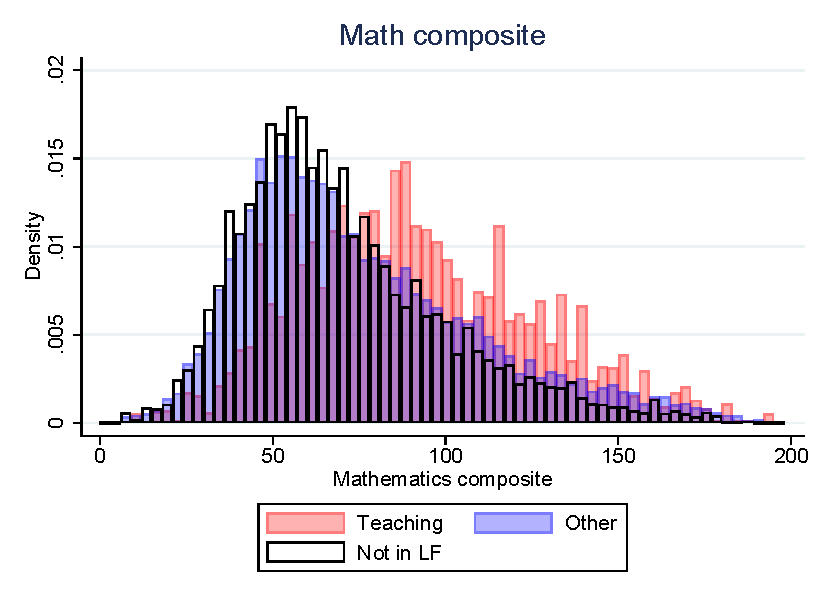
\includegraphics[width=\linewidth]{TALENT_math_occ.pdf}
		\caption{Math} \label{fig:talentmath}
	\end{subfigure}
	\hspace*{\fill} % separation between the subfigures
	\begin{subfigure}{0.49\textwidth}
		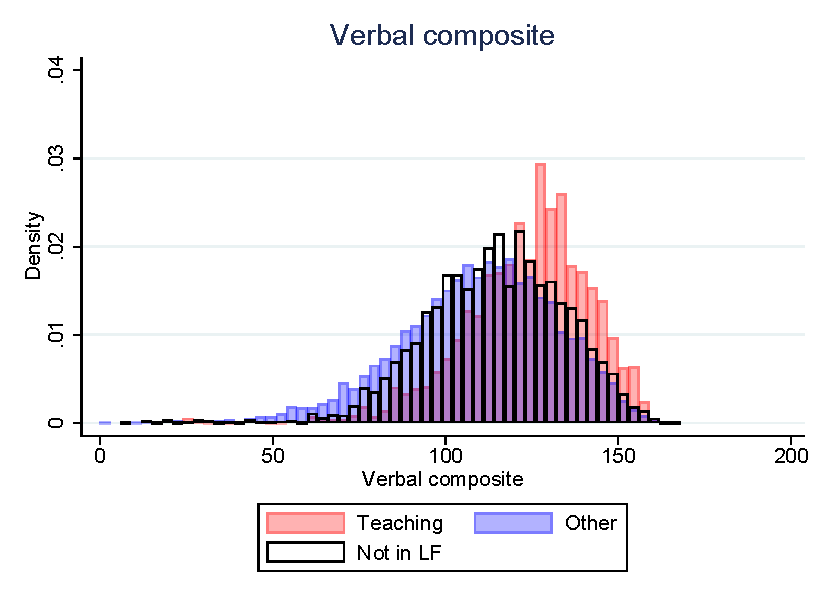
\includegraphics[width=\linewidth]{TALENT_verb_occ.pdf}
		\caption{Verbal} \label{fig:talentverb}
	\end{subfigure}
	\caption{Composite Scores by Occupation in Project TALENT} \label{fig:talent}
\end{figure}

\begin{figure}
	\begin{subfigure}{0.49\textwidth}
		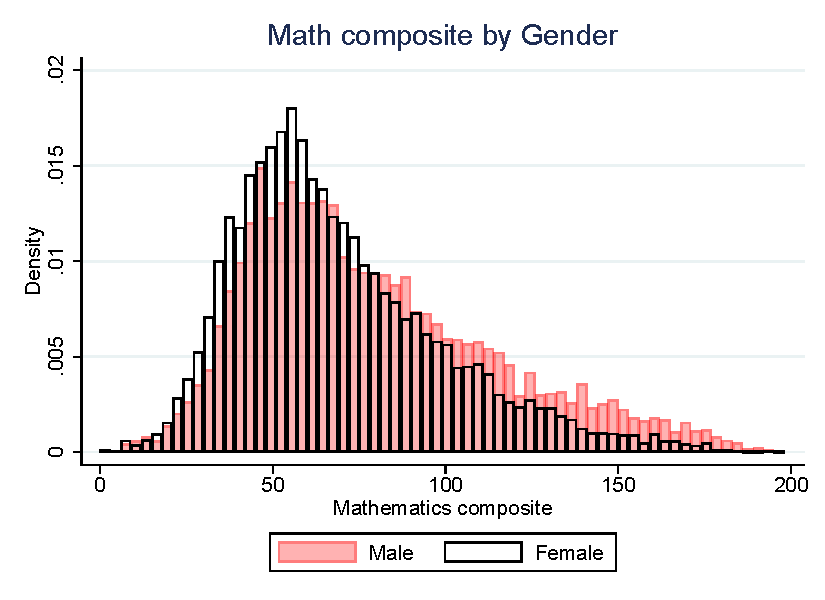
\includegraphics[width=\linewidth]{TALENT_math_by_gender.pdf}
		\caption{Math composite} \label{fig:nlsy79}
	\end{subfigure}
	\hspace*{\fill} % separation between the subfigures
	\begin{subfigure}{0.49\textwidth}
		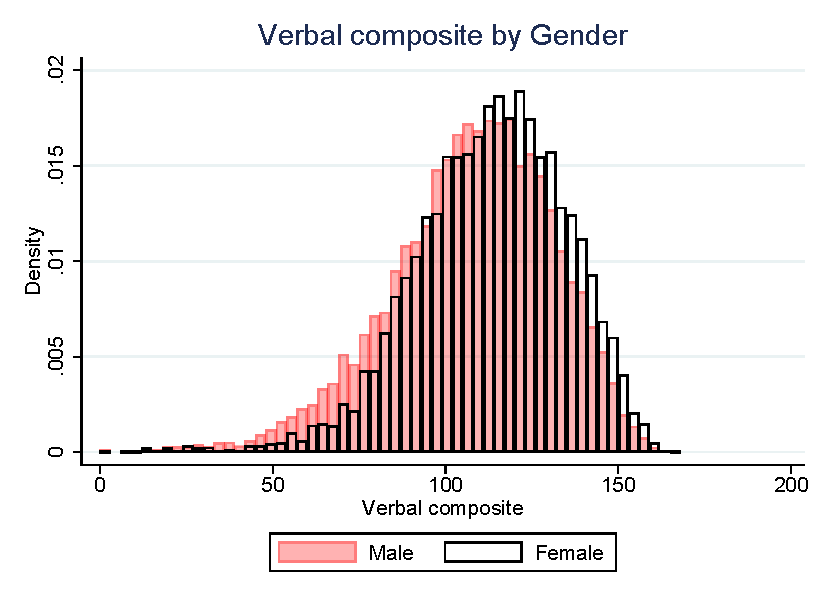
\includegraphics[width=\linewidth]{TALENT_verb_by_gender.pdf}
		\caption{Verbal composite} \label{fig:nlsy97bygender}
	\end{subfigure}
	\caption{Composite Scores by Gender in Project TALENT} \label{fig:talent_gender}
\end{figure}

The distributions of composite IQ scores for Project TALENT respondents split by gender are quite similar (see Figure \ref{fig:IQbygender}). What reconciles Figures \ref{fig:talent}-\ref{fig:IQbygender} is the selection of more talented women into teaching, which we plot in Figure \ref{fig:IQbygenderteach}. Due to the smaller numbers of individuals in Figure \ref{fig:IQbygenderteach} compared to the three previous figures (the number of men is particularly low), the plot contains more noise and one should draw any conclusion with appropriate caution. With this in mind, it does appear that teaching attracts higher-ability individuals and that the selection of women along this dimension is somewhat stronger, plausibly due to the lack of career opportunities in other occupations.

\begin{figure}
	\begin{subfigure}{0.49\textwidth}
	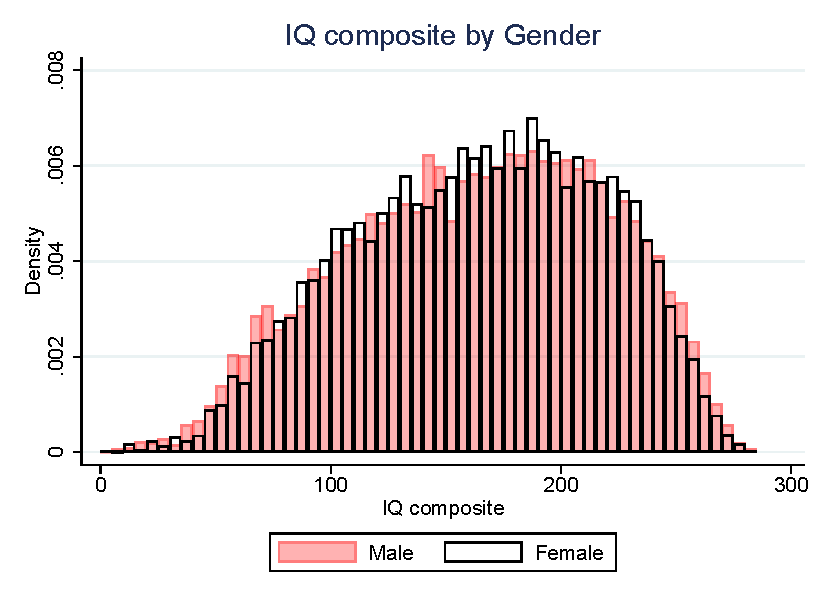
\includegraphics[width=\linewidth]{iq_by_gender.pdf}
	\caption{All Occupations}
	\label{fig:IQbygenderall}
	\end{subfigure}	
	\hspace*{\fill} % separation between the subfigures
	\begin{subfigure}{0.49\textwidth}
	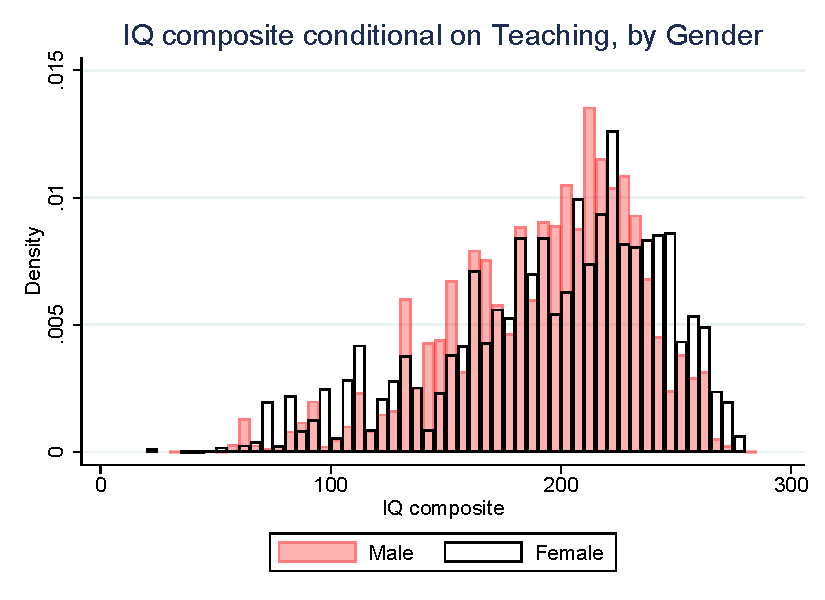
\includegraphics[width=\linewidth]{iq_by_gen_teach.pdf}
	\caption{Teaching Only}
	\label{fig:IQbygenderteach}
	\end{subfigure}
	\caption{Composite IQ Scores by Gender in Project TALENT}
	\label{fig:IQbygender}
\end{figure}

The 11-year follow-up survey provides a snapshot of young workers' occupational choices together with the pre-labor market aptitude profile in the early 1970s. For later years, we use date from the two NLSYs and we will give a brief overview in the next section.

\subsection{NLSY79 and NLSY97}
In contrast to Project TALENT, the two NLSYs initiated in 1979 and 1997 are widely used and many readers are already familiar with the data. \cite{Cooksey:2018}, among many others, provides a comprehensive overview of the two surveys. For the purposes of our paper, the {\it Armed Forces Qualification Test} (AFQT) scores are of particular interest since we need proxies to capture differences in the individuals' raw skills, which is the crucial source of exogenous variation in our model. The score consists of four sections of the {\it Armed Services Vocational Aptitude Battery} (ASVAB): arithmetic reasoning, word knowledge, paragraph comprehension, and numerical operations. The tests took place in 1980 and 1999 for NLSY79 and NLSY97 cohorts, respectively.

Since the tests were administered at different ages (and times) and used different formats, NLS program staff re-normed the scores in 2006, in order to facilitate cross-cohort comparisons.\footnote{\cite{Altonji:2009} also propose a method to enable a comparison of AFQT scores across the two NLSY samples. Note that we cannot construct equivalence scores that would allow as to compare results from aptitude tests in Project TALENT with those from the two NLSYs.} Table \ref{tab:NLSYscores} shows summary statistics for the individuals in our sample, divided into three categories: (1) teachers, (2) non-teachers/others, (3) not in labor force. Since an individual usually has multiple employment spells, she might be in all these categories over the course of the panel. We define an individual as a teacher if she has at least one spell in teaching that is longer than 9 months (one academic year). An individual is out of labor force if she reported to be out of labor force for 208 consecutive weeks for a reason {\it other} than schooling.\footnote{After four years, ``not in the labor force'' is effectively an absorbing state. The probability of returning to the labor force is less than 1\%.}

	\begin{table}[h!]
		\centering
		\begin{tabular}{lccccc}
			\toprule
%			\toprule
			\multicolumn{6}{c}{Panel A: NLSY79}\\
			\midrule
%			& (1) & (2) & (3)\\
			& \multirow{2}{*}{Teachers} & \multirow{2}{*}{Other} & \multirow{2}{*}{Unemployed} & Not in & \multirow{2}{*}{Total}\\
			& &  &  & Labor Force & \\
			\midrule
			Female & 999 & 2,933 & 221 & 1,568 & 5,721\\
			\quad (\% of subsample) & (43.19\%) & (44.85\%) & (41.39\%) & (76.34\%) & (50.01\%)\\
			\midrule
			Math ability & 2.450 & 2.443 & 1.919 & 1.962 & 2.334\\
			\quad (st.dev.) & (0.932) & (1.018) & (0.935) & (0.912) & (1)\\
			\midrule
			Verbal ability & 3.614 & 3.509 & 2.920 & 3.057 &  3.422\\
			\quad (st.dev.) & (0.864) & (0.971) & (1.088) & (1.074) & (1)\\
			\midrule
			Social ability & 3.891 & 3.824 & 3.566 & 3.552 & 3.777\\
			\quad (st.dev.) & (1.016) & (0.980) & (0.969) & (1.011) & (1)\\
			\midrule
			AFQT & 1.780 &  1.741 & 1.184 & 1.270 & 1.638\\
			\quad (st.dev.) & (0.928) & (1.004) & (0.950) & (0.956) & (1)\\
			\midrule
			Observations &  2,313 & 6,539 &  534 & 2,054 & 11,440\\
			\quad (\% of total sample) & (20.22\%) & (57.16\%) & (4.67\%) & (17.95\%) & (100.00\%)\\
			\bottomrule
%			\bottomrule
			\\
			\toprule
%			\toprule
			\multicolumn{6}{c}{Panel B: NLSY97}\\
			\midrule
			& \multirow{2}{*}{Teachers} & \multirow{2}{*}{Other} & \multirow{2}{*}{Unemployed} & Not in & \multirow{2}{*}{Total}\\
			& &  &  & Labor Force & \\
			\midrule
			Female & 478 & 2,184 & 171 & 605 & 3,438\\
			\quad (\% of subsample) & (48.53\%) & (46.60\%) & (48.03\%) & (64.71\%) & (49.38\%)\\
			\midrule
			Math ability & 1.309 & 1.422 & 1.710 & 1.780 & 1.469\\
			\quad (st.dev.) & (0.885) & (0.959) & (1.148) & (1.164) & (1)\\
			\midrule
			Verbal ability & 1.475 & 1.590 & 1.985 & 2.001 &  1.649\\
			\quad (st.dev.) & (0.879) & (0.957) & (1.144) & (1.154) & (1)\\
			\midrule
			Social ability & 5.684 & 5.645 & 5.478 & 5.460 & 5.614\\
			\quad (st.dev.) & (0.904) & (0.967) & (1.108) & (1.158) & (1)\\
			\midrule
			AFQT & 1.776 & 1.665 & 1.045 & 1.185 & 1.585\\
			\quad (st.dev.) & (0.943) & (0.998) & (0.808) & (0.961) & (1)\\
			\midrule
			Observations &  985 & 4,687 &  356 & 935 & 6,963\\
			\quad (\% of total sample) & (14.15\%) & (67.31\%) & (5.11\%) & (13.43\%) & (100.00\%)\\
			\bottomrule
%			\bottomrule			
		\end{tabular}
		\caption{NLSY Scores by Occupation}
		\label{tab:NLSYscores}
	\end{table}
	
If indeed labor market barriers are shrinking over time, we would expect to see some evidence of this in the occupational choice of women in more recent cohorts and hence in the NLSY79 and NLSY97. In these younger cohorts, the share of women among teachers continues to be high. The gender composition of teachers in NLSY 79 is comparable to the one we observe in Project TALENT. In the more recent NLSY 97, the share is a few percentage points lower. In contrast, the share of female workers in other occupations is rising, from approximately 39 percent in Project TALENT to 44 percent in NLSY79, and 45 percent in NLSY97. The gender composition of those who are out of the labor force is heading in the opposite direction. It dropped to 66 percent among NLSY79 respondents and 64 percent among NLSY97 respondents, compared to almost 80 percent in the 11-year post graduation survey from Project TALENT.

One significant difference between the Project TALENT and NLSY respondents are the aptitude scores for those who are not in the labor force. While their average score was {\it higher} than the average score of those in {\it Other} in Project TALENT, the ranking is reversed in the two NLSYs. This suggests that the exit rate from ``not in the labor force'' is correlated with the respondents' ability. High and low ability individuals appear to respond differentially to changes in labor market discrimination and this is further corroborated in a set of plots we present below. 

Figure \ref{fig:nlsy_by_occ} plots the NLSY analogues of the math and verbal scores in Project TALENT shown in Figure \ref{fig:talent}. Clearly, teaching still attracts higher-ability individuals than ``other'' occupations or those who are not in the labor force. While the ability distribution of teachers still first-order dominates the scores in ``other'' occupations in the 1979 survey, there is a remarkable shift in the talent distribution of those who are not in the labor force. It is for more right-skewed than the distribution of workers in ``other'' occupations. Unfortunately, the 1997 data is considerably more noisy mostly due to the smaller sample size and we're refraining from reading too much into any particular feature of the data. This being said, it is worth highlighting that the definition of ``not in the labor force'' is {\it not} identical in the TALENT data on the one hand and the NLSY data on the other.\footnote{The difference stems from the fact that we observe Project TALENT participants relatively infrequently and the respondents' labor market histories are less complete.} It is, however, suggestive of a trend whereby high-ability individuals are pulled into the labor force more ``aggressively'' compared to low-skill workers over time.

\begin{figure}
	\begin{subfigure}{0.49\textwidth}
		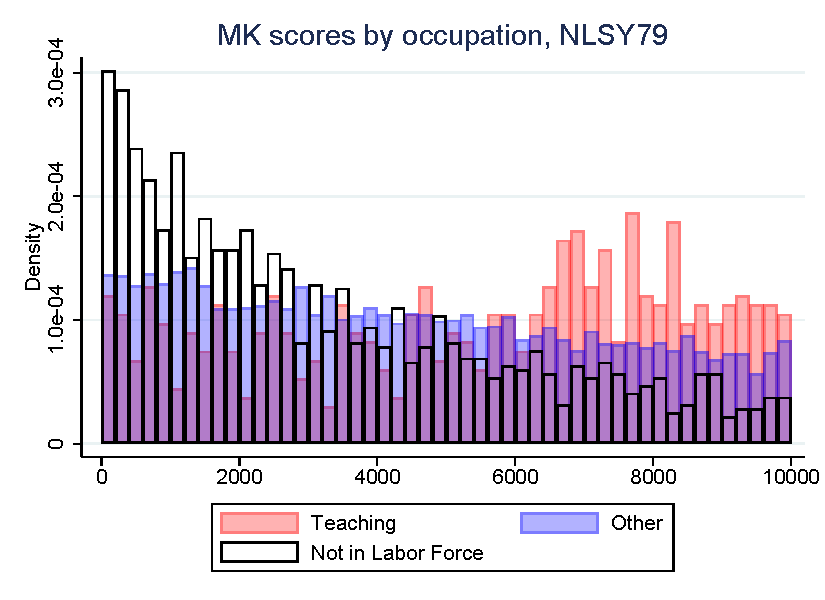
\includegraphics[width=\linewidth]{NLSY79_MK_occ.pdf}
		\caption{Math Knowledge (NLSY79)} \label{fig:nlsy79math}
	\end{subfigure}
	\hspace*{\fill} % separation between the subfigures
	\begin{subfigure}{0.49\textwidth}
		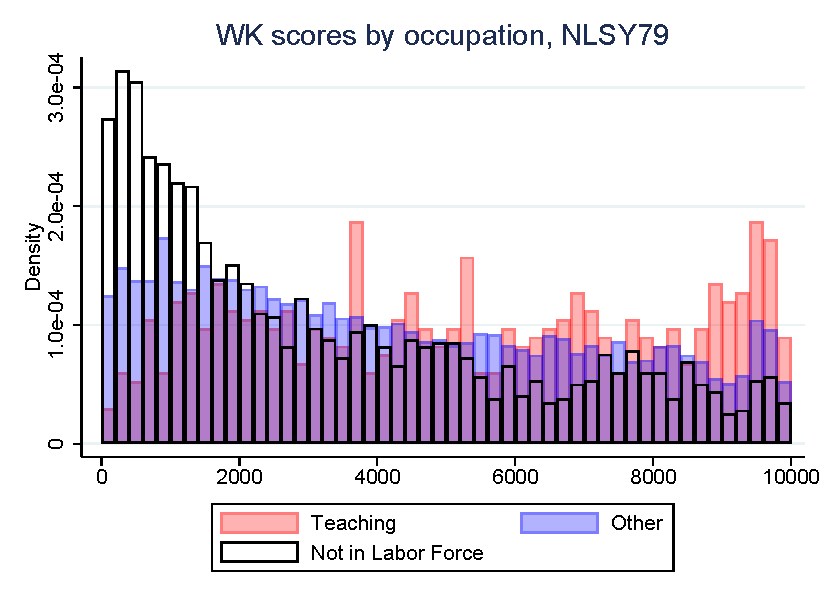
\includegraphics[width=\linewidth]{NLSY79_WK_occ.pdf}
		\caption{Word Knowledge (NLSY79)} \label{fig:nlsy79word}
	\end{subfigure}
		\begin{subfigure}{0.49\textwidth}
		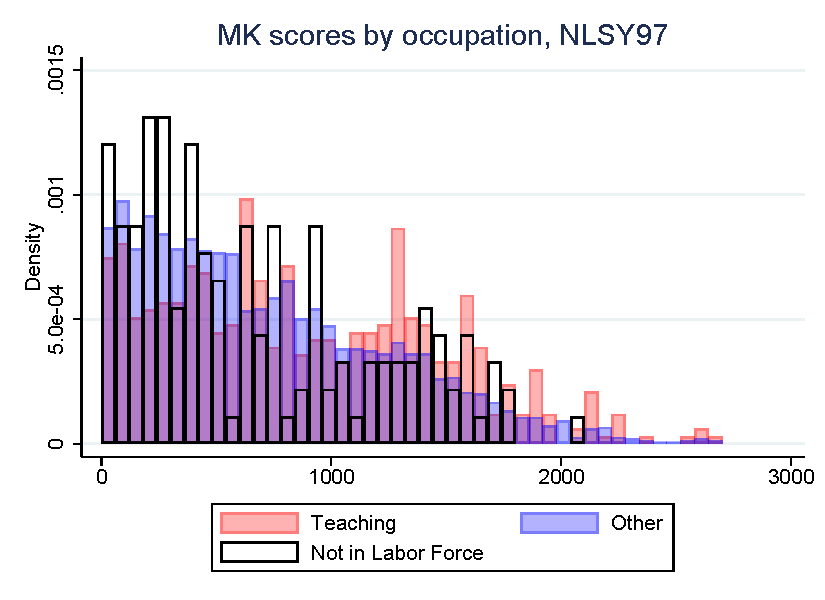
\includegraphics[width=\linewidth]{NLSY97_MK_occ.pdf}
		\caption{Math Knowledge (NLSY97)} \label{fig:nlsy97math}
	\end{subfigure}
	\hspace*{\fill} % separation between the subfigures
	\begin{subfigure}{0.49\textwidth}
		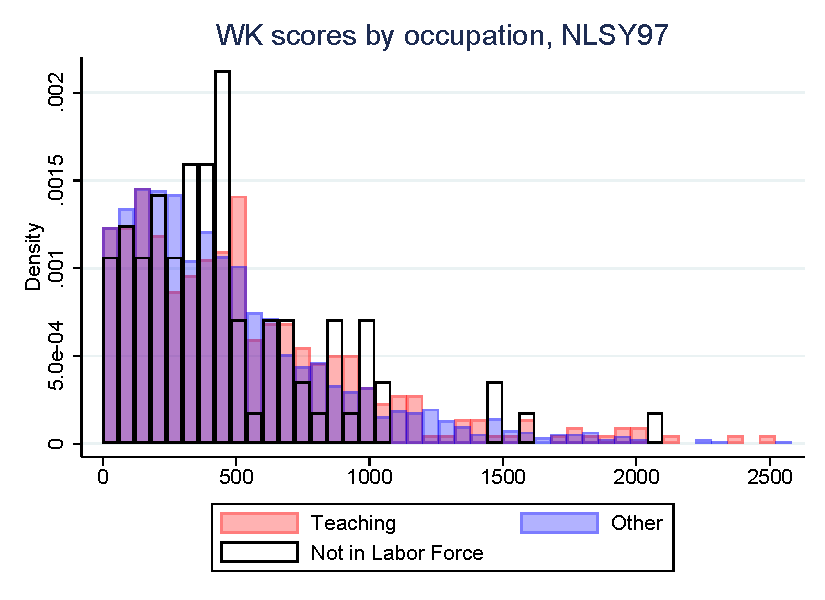
\includegraphics[width=\linewidth]{NLSY97_WK_occ.pdf}
		\caption{Word Knowledge (NLSY97)} \label{fig:nlsy97wprd}
	\end{subfigure}

	\caption{AFQT Scores by Occupations}
	\label{fig:nlsy_by_occ}
\end{figure}

%\begin{figure}
%	\begin{subfigure}{0.49\textwidth}
%		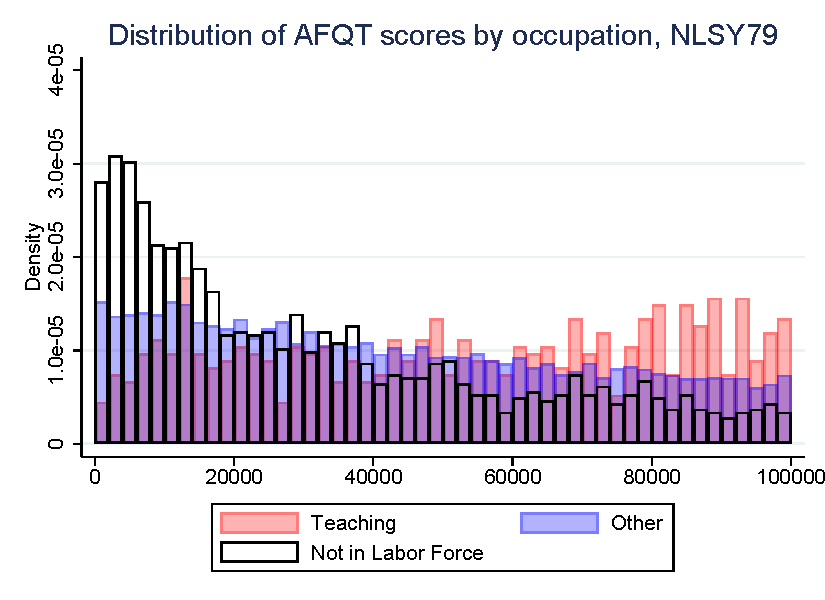
\includegraphics[width=\linewidth]{NLSY79_afqt79_occ_new.pdf}
%		\caption{NLSY79} \label{fig:nlsy79}
%	\end{subfigure}
%	\hspace*{\fill} % separation between the subfigures
%	\begin{subfigure}{0.49\textwidth}
%		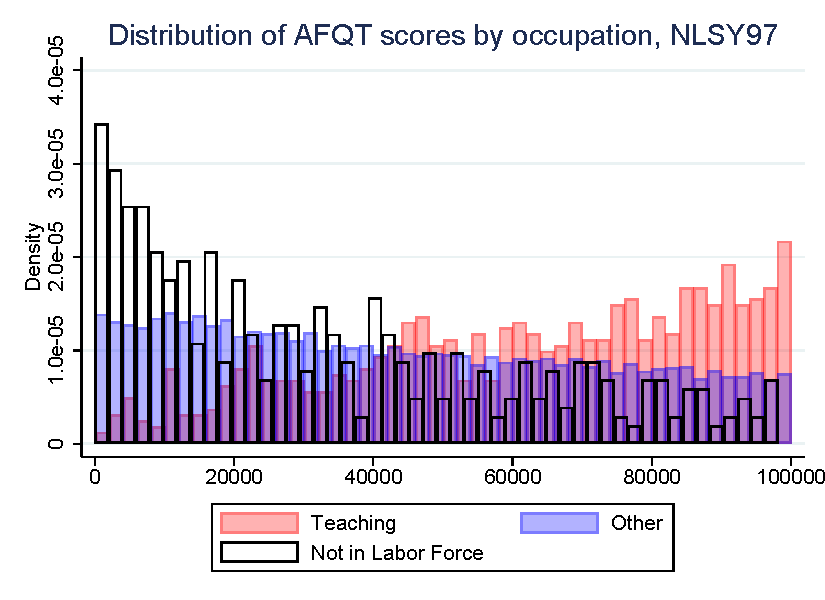
\includegraphics[width=\linewidth]{NLSY97_afqt97_occ_new.pdf}
%		\caption{NLSY97} \label{fig:nlsy97}
%	\end{subfigure}
%	\caption{Distribution of AFQT Scores by Occupations}
%	\label{fig:nlsy}
%\end{figure}

Figures \ref{fig:nlsy_by_gender}-\ref{fig:nlsy_comp_by_gender} are the NLSY analogues of Figures \ref{fig:talent_gender}-\ref{fig:IQbygender}.

\begin{figure}
	\begin{subfigure}{0.49\textwidth}
		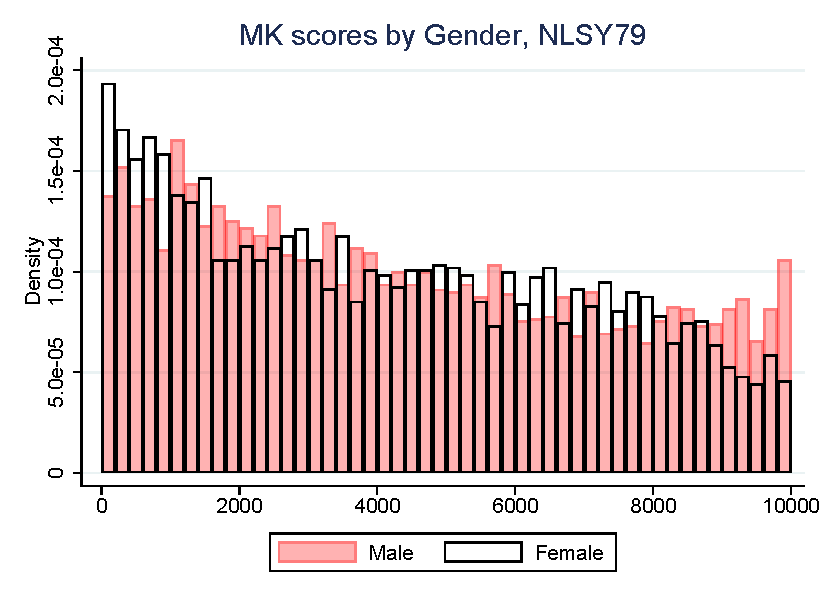
\includegraphics[width=\linewidth]{NLSY79_MK_gender.pdf}
		\caption{Math Knowledge (NLSY79)} \label{fig:nlsy79math}
	\end{subfigure}
	\hspace*{\fill} % separation between the subfigures
	\begin{subfigure}{0.49\textwidth}
		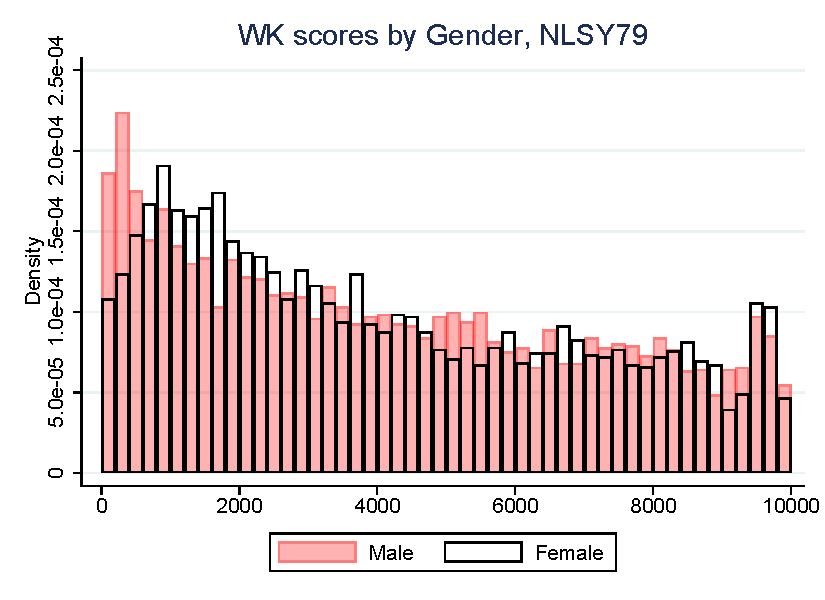
\includegraphics[width=\linewidth]{NLSY79_WK_gender.pdf}
		\caption{Word Knowledge (NLSY79)} \label{fig:nlsy79word}
	\end{subfigure}
		\begin{subfigure}{0.49\textwidth}
		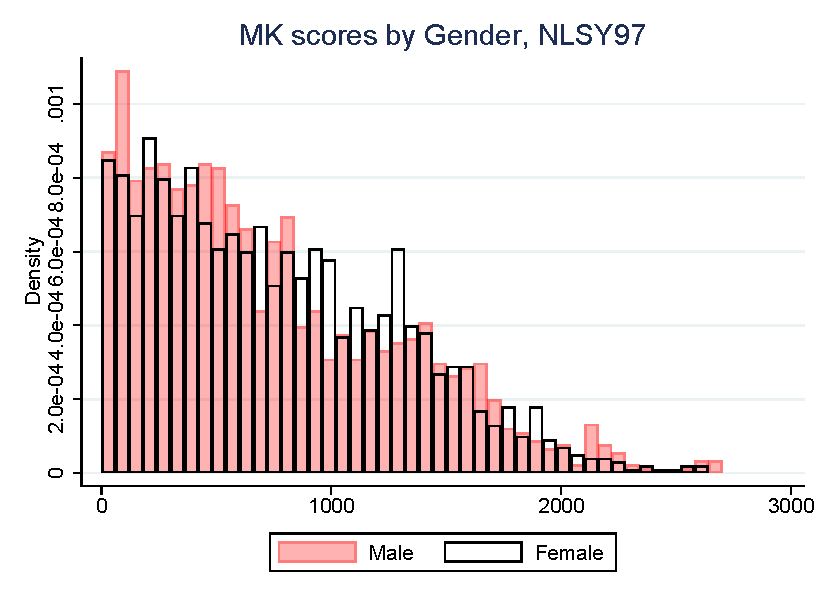
\includegraphics[width=\linewidth]{NLSY97_MK_gender.pdf}
		\caption{Math Knowledge (NLSY97)} \label{fig:nlsy97math}
	\end{subfigure}
	\hspace*{\fill} % separation between the subfigures
	\begin{subfigure}{0.49\textwidth}
		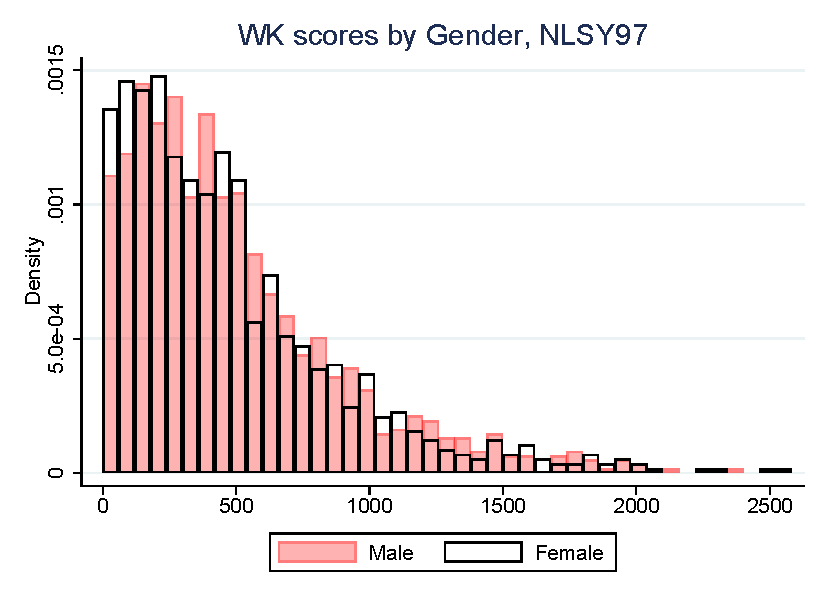
\includegraphics[width=\linewidth]{NLSY97_WK_gender.pdf}
		\caption{Word Knowledge (NLSY97)} \label{fig:nlsy97wprd}
	\end{subfigure}

	\caption{Topic Scores by Gender}
	\label{fig:nlsy_by_gender}
\end{figure}

\begin{figure}
	\begin{subfigure}{0.49\textwidth}
		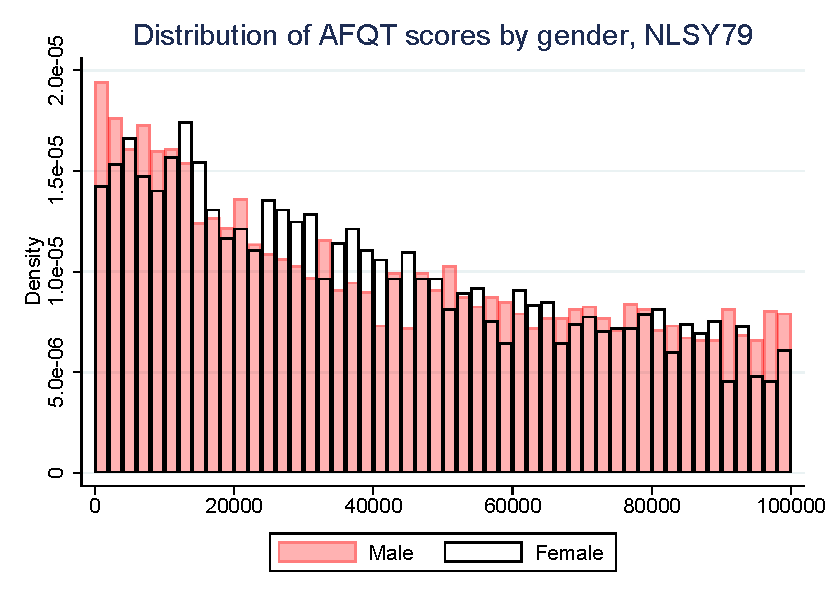
\includegraphics[width=\linewidth]{NLSY79_afqt79_gender.pdf}
		\caption{AFQT Composite (NLSY79)} \label{fig:nlsy79math}
	\end{subfigure}
	\hspace*{\fill} % separation between the subfigures
	\begin{subfigure}{0.49\textwidth}
		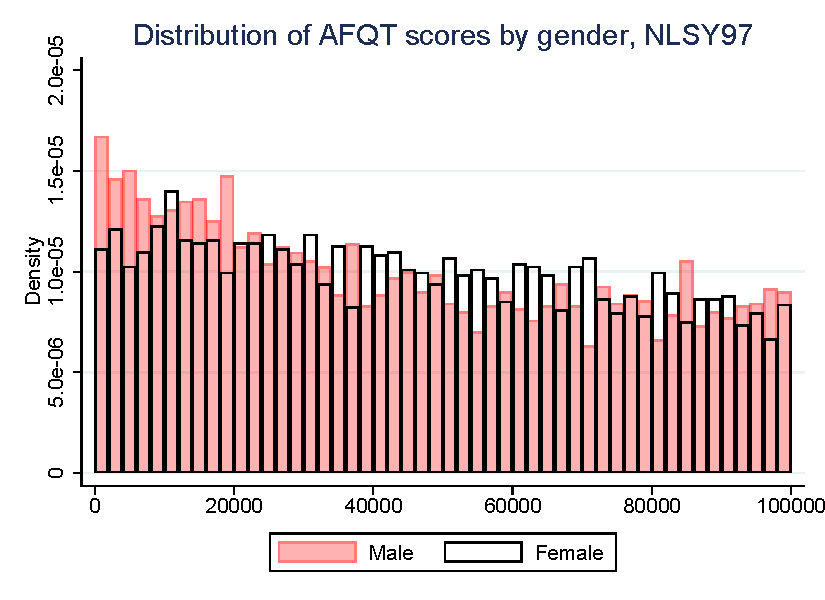
\includegraphics[width=\linewidth]{NLSY97_afqt97_gender.pdf}
		\caption{AFQT Composite (NLSY97)} \label{fig:nlsy79word}
	\end{subfigure}
	\caption{AFQT Scores by Gender}
	\label{fig:nlsy_comp_by_gender}
\end{figure}
	
Unfortunately, the composite score distributions aren't comparable between Project TALENT and NLSY cohorts for several reasons. Although the ability tests try to capture math and verbal abilities, the tests themselves are very different. Therefore, it is impossible to compare changes in score distributions over time. Despite this limitation we can still compare the composition (by gender or occupation) {\it within} cohorts across the three surveys. In fact, the particular {\it Roy} flavor of our model suggests that this is where the interesting action is.

Differences in the frequency of the surveys further complicate comparisons between Project TALENT and the NLSY's. The NLSY79 and NLSY97 survey the respondents far more frequently and this enables us to construct more detailed employment histories and occupation choices over the course of panels. While Project TALENT provides data on the respondents' {\it current} occupation in the 1, 5, and 11-year post waves, it misses some of the higher-frequency churn since it doesn't ask any retrospective career questions. Moreover, the probability of being a teacher one year after high school graduation is vanishingly small (0.08\% of the sample). In the figures and tables presented so far we report the occupations reported in the 11-year follow-up study. While certainly less complete than the NLSY data, Project TALENT still offers insights into the career decisions of young adults at a time for which there is only a very limited supply of nationally representative longitudinal survey data.\footnote{In ongoing work, we synthetically impose some of the data limitations in Project TALENT on the NLSY in order to get a better sense for underlying changes in labor market conditions and career decisions across cohorts. Evidently we're giving up some valuable details in the process for the benefit of more cross-survey comparability.}

Project TALENT, NLSY79, and NLSY97 provide us with the data moments that we match to model-generated moments in order to quantify the static and dynamic effects of the implied educational barriers and labor market barriers. While the discussion so far emphasized the contrast between men and women, it is worth emphasizing that our model framework can accommodate more richness in terms of the salient groups of workers. In ongoing work we are incorporating race and ethnicity to more fully capture the salient educational and labor market frictions in the data.\footnote{Since the racial categorization is somewhat problematic in Project TALENT, this extension poses additional challenges.}

The final element in our calibration element relies on O*Net's characterization of occupation-specific skill requirements. We use a three-dimensional job characterization: mathematics, verbal, and social. We decompose the requirements of each job into an absolute and a comparative dimension in a way that aligns naturally with the notion of absolute and comparative advantage.

We characterize the comparative requirements by a triple of weights based on the dimension-by-dimension skill ranking of each job. To account for the possibility that jobs with similar comparative profiles are characterized by different overall skill intensities, we also create an absolute profile based on the weighted sum of skill-specific rankings. Given the non-linearity of payoffs in our model, the distinction between comparative and absolute advantage is critical for our calibration strategy\footnote{In this respect, our model differs from a plain-vanilla occupational choice model \`a la \cite{Roy:1951}.}

Last but not least, we use these skill profiles to project the survey respondents' three-dimensional abilities into an $I$-dimensional vector of job-specific abilities.

%{\sc This is currently work in progress!}

%\section{First Best Allocation}\label{sec:firstbest}
% \section{Decentralized Competitive Equilibrium (No Frictions) }\label{sec:firstbest}
% In order to highlight the mechanisms that govern the individuals' occupational choice we first solve for a decentralized equilibrium that implements the optimal allocation of adults to ``teaching'' and ``other'' in a single location. Put differently, we solve the model for a wage profile $\omega^*(h^T)$ that pays teachers with human capital $h^T$ their marginal product.\footnote{In section \ref{sec:model} we specified the model for an arbitrary profile $\omega$. Here we impose further restrictions on this function.}

% How can we characterize the teacher's marginal product? Recall that only workers produce the final (consumption) good using a linear production function with productivity $A^O$. Thanks to stable random matching of students to teachers the ability distribution of students is identical across class rooms and a teacher's marginal value only varies with the number of students in her class room, denoted by $N(h^t)$. Clearly, then, the wage profile is linear in $N(\cdot)$. Since $N$ is not linear in $h^T$ in general this implies that the wage profile is not linear in $h^T$ either.

% Since teachers are compensated for the incremental human capital in ``other'', we could characterize the teacher's wage profile.
% \begin{prp}[Teacher's wage profile] For a given teacher with human capital $h^T$ and aggregate human capital in teaching $\widetilde{H}^T$, the wage in teaching is proportional to the \textit{number of students} in the teacher's class and is characterized by
% \begin{align}
% \label{eq:omegaOpt}
%   \omega(h^T,\widetilde{H}^T) & =  \frac{\overbrace{{H'}^O {A'}^O}^{\textrm{total output (next period)}}}{\underbrace{\int_0^\infty f^O(a) da}_{\begin{subarray}{c}\textrm{fraction of prospective} \\ \textrm{production workers in class}\end{subarray}}} \underbrace{\frac{\left( h^T \right)^{\frac{\beta}{\sigma}}}{{\widetilde{H}^T}}}_{\textrm{fraction of students taught}}
% \end{align}
% where
% \begin{align*}
% \label{}
% %  \widetilde{H'}^{T} & = \int_0^\infty \left(\left(\tfrac{2 \widetilde{H}^T}{M}\right)^\sigma a^\alpha s^T\left(a,\widetilde{H}^T\right)^\phi e^T(a,\widetilde{H}^T)^\eta \right)^{\frac{\beta}{\sigma}} f^T(a) da
%   \widetilde{H'}^{T} & = \int_0^\infty {h^T}^{\frac{\beta}{\sigma}} f^T(a) da
% \end{align*}
% is the ${\left( \tfrac{\beta}{\sigma} \right)}^{\textrm{th}}$ moment of the distribution of human capital among current teachers.
% \end{prp}

% The second term in equation \eqref{eq:omegaOpt} captures the idea that a teacher's wage depends on class size, which is a non-linear function of her human capital $h^T$. Recall from equations \eqref{eq:sT} and \eqref{eq:eT} that a prospective teacher's optimal $s^T$ and $e^T$ depends on the quality of today's teachers (i.e.~their human capital) and on the slope of the wage profile next period and hence on both today's $ \widetilde{H}^{T}$ as well as tomorrow's $\widetilde{H'}^{T}$.

%\section{Constrained Optimal Allocation}
% \section{Decentralized Competitive Equilibrium with Educational Barriers and Labor Market Discrimination}
% To highlight the effect of educational barriers and labor market discrimination we add group- and occupation-specific distortions to the model in section \ref{sec:firstbest}. This is mostly a heuristic exercise since parsimony of our state space enables us to characterize the full transition path from one set of distortions to another. We highlight this feature of the model here since there have arguably been secular changes in educational barriers and labor market distortions for groups other than white males. To fix ideas, however, we simply compare steady states associated with particular wedges $\tau$ indexed by $\omega$ (for labor market discrimination), $e$ (for educational barriers), and $g$ for groups (race, gender,\ldots).

% We can show that this economy has a steady state in $H^T$ and we can characterize it in a single equation:
% \begin{equation}
% \label{ }
% \textrm{To Be Inserted!}
% \end{equation}

% Moreover, the occupational choice boundary, denoted $\bar{a}^T(a^O)$ depends on the magnitude of the educational barriers and labor market frictions, but not current or future aggregate human capital in teaching. The boundary can be characterized implicitly by the following condition:

% \begin{eqnarray}
% \label{eq:occChoice}
% \left(\frac{1-{\tau'}^{O,w}}{1-{\tau'}^{T,w}}\right) \left(\frac{1-\eta}{1-\tfrac{\eta\beta}{\sigma}}\right)  \left(\frac{1-s^{O}}{1-s^{T}}\right)^{\frac{1}{\mu}}  \left(\frac{(a^O)^\frac{\alpha}{1-\eta}}{\big({\bar{a}^T(a^O)}\big)^\frac{\alpha}{\frac{\sigma}{\beta}-\eta}} \right) \nonumber \\
% = \left(\frac{\int_0^\infty a^\frac{\alpha}{1-\eta} {f^O(a)} da}{\int_0^\infty {f^O(a)} da} \right) \left(\int_0^\infty a^\frac{\alpha}{\frac{\sigma}{\beta}-\eta} {f^T(a)} da\right)^{-1} 
% \end{eqnarray}


% The calibration in section \ref{sec:quant} will go beyond the simple comparative statics here and match moments along the secular transition from the late 1960s to the more recent past.

%{\sc This is work in progress!}
%\section{Model Extension with $L > 1$ Locations}
%In section \ref{sec:model} we motivated lump-sum taxation by the stylized fact that school districts are, to a considerable extent, funded by local property taxes. It is therefore natural to consider multiple locations with distinct taxes $\{T_1,\ldots,T_L\}$. In this version of the model, young agents not only decide which career path they would like to pursue, but they also choose a location for their education. % NOTE TO SELF: HOW DO WE RULE OUT THAT KIDS MOVE TO HIGH TAX AREAS FOR THEIR EDUCATION AND THEN RE-LOCATE TO LOW TAX LOCATIONS IN ADULTHOOD.
%The assumption of a single location with (stable) random matching between students and teachers had the benefit of tractability. The aggregate state of the economy could be summarized by a single scalar, $ \widetilde{H}^{T}$.
%
%Abandoning the assumption of random student assignment implies that the aggregate state is now given by an entire distribution of $\widetilde{h}^{T}$ rather than a single moment of that same distribution. This turns out be a rather challenging generalization. What appears to be more relevant empirically is the introduction of multiple locations, differentiated by local (lump sum) tax levels and possibly some (as of yet) unspecified amenity. As long as we maintain the assumption of effectively random student-teacher assignment within locations, we can rely on tools from \cite{Lucas:2014} and more recently used in \cite{Martellini:2019} to keep the state space small enough and thus the dynamic program tractable.
%
%This model extension enables us to capture the quantitative effects associated with the salient stylized fact of increasing socio-economic segregation of students -- and plausibly even teachers -- between inner cities and suburbs.
%
%{\sc This is currently work in progress!}
\section{Quantitative Analysis}\label{sec:quant}
\subsection{Calibration Strategy}\label{sec:calstrat}
The model allows analyzing the effects of changes in the labor market barriers. The aim of the calibration is to parametrize the economy to match aggregate and micro moments that characterize the US economy in 1970, 1990, and 2010 to their model counterparts. We select these years since the respondents from Project TALENT, NLSY79, and NLSY97 are, on average, 29 years old. This parameterization will treat these three target years as steady states of the model.

We assume that the idiosyncratic occupation-specific abilities are distributed log-normal and the relative innate talent levels are identical across all groups. Tables \ref{tab:assump}-\ref{tab:calibr} summarize the elements of a sample parameterization. Table \ref{tab:assump} summarizes the assumptions and normalization for our base parameterization of the model. We assume that there are no labor and human capital barriers for men in all occupations. We also assume that labor and human capital barriers in home production are zero for all groups.

Table \ref{tab:param} summarizes the key parameters. Table \ref{tab:calibr} presents the endogenous variables and their targeted empirical counterparts. Parameter value for $\frac{\beta}{\sigma}$ is a crucial parameter that governs how skill distribution changes with respect to the changes in the barriers. Identification of this parameter allows calibrating the model to the data and conduct quantitative and counterfactual analysis. Another parameter that governs how selection into teaching career responds to the changes in the barriers is $\eta$. If $\eta<1$, a decrease in barriers in other occupations leads to the higher occupational threshold, making teaching career more selective. If $\eta>1$, a decrease in barriers in other occupations results in the lower occupational threshold.
%Table \ref{tab:mom} compares the data and the model's predictions.

	\begin{table}[h!]
		\centering
		\begin{tabular}{lccc}
			\toprule
			\toprule
			Parameter & Definition & Determination & Value\\
			\midrule
			$\tau^{w}_{i,men}$ & Labor market barriers for men & Assumption & 0\\
			$\tau^{e}_{i,men}$ & Human capital barriers for men & Assumption & 0\\
			$\tau^{w}_{T,g}$ & Labor market barriers for all groups & Assumption & 0\\
			$\tau^{e}_{T,g}$ & Human capital barriers for all groups & Assumption & 0\\
			$\tau^{e}_{i,g}$ & Human capital barriers for other groups & Normalization & 0\\
			$A_{T}$ & Teachers productivity & Normalization & 1\\
			$\mu_a$ & Mean ability distribution & Normalization & 0\\
			$\sigma_a$ & St.dev. ability distribution & Normalization & 1\\
			\bottomrule
%			\bottomrule
		\end{tabular}
		\caption{Assumptions and Normalization}
		\label{tab:assump}
	\end{table}
	
	\begin{table}[h!]
		\centering
		\begin{tabular}{lcc}
			\toprule
			\toprule
			Parameter & Definition & Determination\\
			\midrule
			$\alpha$ & Ability elasticity of human capital & Wage dispersion \\
			$\eta$ & Goods elasticity of human capital & Aggregate education spending share  \\
			$\phi$ & Time elasticity of human capital & Mincerian return to education for other \\
			$A_{i}$ & Occupation-specific productivity & Labor market shares for men\\
			$\tau^{w}_{i,g}$ & Labor market barriers for other groups & Group gap by occupation\\
			% s_T/s_O, where  s_i=years of school/25 years
			\bottomrule
%			\bottomrule
		\end{tabular}
		\caption{Baseline Parameter Values}
		\label{tab:param}
	\end{table}
	
		\begin{table}[h!]
		\centering
		\begin{tabular}{lcc}
			\toprule
			\toprule
			Parameter & Definition & Empirical Targets\\
			\midrule
			$\beta$ & Teacher elasticity of human capital & Skill composition by occupation and group \\
			$\sigma$ & Class size elasticity of human capital & Normalization to 1\\
			\multirow{2}{*}{$\mu$} &  Trade-off between consumption and & Schooling of teachers relative\\
			& time spent accumulating human capital & to schooling of others\\
			$\lambda_m$ & Scale for male labor market wedges & Share of teachers among men\\
		    $\lambda_f$ & Scale for other group labor market wedges & Share of teachers among other group\\
			\bottomrule
%			\bottomrule
		\end{tabular}
		\caption{Benchmark Calibration}
		\label{tab:calibr}
	\end{table}
	
% 	\begin{table}[h!]
% 		\centering
% 		\begin{tabular}{lcc}
% 			\toprule
% 			\toprule
% 			Moments & Model & Data \\
% 			\midrule
% 			& & \\
% 			& & \\
% 			\bottomrule
% %			\bottomrule
% 		\end{tabular}
% 		\caption{Model and Data Moments}
% 		\label{tab:mom}
% 	\end{table}
	
%$\frac{s_O}{s_T}=\frac{\mu \phi+\frac{\beta}{\sigma}-\eta}{\mu \phi+1-\eta}=1-\frac{1-\frac{\beta}{\sigma}}{\mu \phi+1-\eta}$


%\subsection{Counterfactual Experiments}
%{\sc To Be Completed!}
\newpage
\section{Conclusion}\label{sec:conclusion}
This paper develops a novel occupational choice model that captures the distinct nature of teaching and learning -- and hence human capital accumulation. In addition to the static gains and losses associated with labor market distortions and educational barriers, we can characterize the dynamic effects that are driven by the number and ability of workers who are drawn to the teaching profession. This occupational choice, in turn, shapes the incentives to invest in human capital when the agents are young, i.e. when they are students.

The model also introduces wage profiles that are non-linear in the workers' human capital and this generalization implies that occupational choice is driven by {\it comparative} as well as {\it absolute} advantages across the various occupations. This is a significant departure from the canonical occupational choice models in the spirit of \cite{Roy:1951}. At this point, the extent of this non-linearity is not pinned down precisely and this is an area of ongoing work.

The model reconciles several salient stylized facts. In addition to the change in the student-teacher ratios and per-student-expenditures mentioned above, they are: (1) the increase in the share of women in teaching jobs from 4.6 percent in 1970 to 6.7 percent in 2010; (2) the drop in the share of men who are teachers from 2.9 percent to 2.1 percent during that same time; (3) the sharp rise in the female labor force participation rate; (4) the slight decline in the male labor force participation rate; and (5) the evolution of the skill composition by gender and occupation between 1970 and 2010.

The somewhat loose discussion of our calibration strategy in section \ref{sec:calstrat} reflects the work-in-progress nature of our quantitative exercise. The model is otherwise well identified and in ongoing work we are calibrating the remaining parameters to match the salient moments at three different points in time: 1970, 1990, and 2010. We select these years since the respondents from all three longitudinal surveys are, on average, 29 years old. This parameterization will treat these three target years as steady states of the model. Future work will explore the human capital transition dynamics between steady states.
%\begin{enumerate}
%    \item Reported some data patterns;
%    \item Developed a theoretical model;
%    \item Outlined calibration strategy which we leave for further analysis;
%    \item Next step is to use the model to characterize the US economy in 1970, 1990, and 2010, as well as transition dynamics between these years.
%\end{enumerate}



\newpage
\bibliography{/Users/simeonalder/Dropbox/Bibliography/MasterBibliography}
\bibliographystyle{ecta}



% \newpage
% \begin{align}
% \beta < 1-\eta \textit{\,to guarantee existence of stable\,} \widetilde{H^T} = \widetilde{H^T}' > 0 \nonumber\\
% \tfrac{\sigma}{\beta} > \eta \textit{\,and\,} \mu \phi > 0 \textit{\,for\,} s^{T*} \in (0,1) \nonumber\\
% 1 > \eta \textit{\,and\,} \mu \phi > 0 \textit{\,for\,} s^{O*} \in (0,1) \nonumber
% \end{align}

\end{document}
